\chapter{Πειράματα και Αποτελέσματα} \label{Chapter5}
Στο παρόν κεφάλαιο παρουσιάζονται τα πειράματα και τα αποτελέσματα που πραγματοποιήθηκαν για την επαλήθευση και την αξιολόγηση της συμπεριφοράς των υποσυστημάτων της ρομποτικής πλατφόρμας Monstertruck, σε σχέση με την επιθυμητή. Παράλληλα, πραγματοποιείται και σύγκριση μεταξύ των διαφορετικών εκδοχών ορισμένων υποσυστημάτων, όπως αυτά παρουσιάστηκαν στο Κεφάλαιο \ref{Chapter4}. 

\bigskip
Η εκτέλεση των πειραμάτων πραγματοποιήθηκε, μέσω προσομοίωσης σε δύο διαστάσεις με τον προσομοιωτή STDR, σε τρεις διαστάσεις με τον προσομοιωτή Gazebo, όπως επίσης και στο φυσικό ρομπότ που αναπτύχθηκε στα πλαίσια της παρούσας διπλωματικής. Τα εν λόγω πειράματα εκτελέστηκαν σε επίπεδο προσομοίωσης σε έναν υπολογιστή με επεξεργαστή Intel Core i5 2.4GHz, 6GB RAM και κάρτα γραφικών NVIDIA GeForce GT330M, ενώ σε επίπεδο φυσικού ρομπότ σε έναν υπολογιστή ODROID-XU4 με προδιαγραφές, όπως αυτές παρουσιάστηκαν στον πίνακα \ref{tab:computer_specs}, όπου και τα δύο υπολογιστικά συστήματα έτρεχαν το λειτουργικό σύστημα Ubuntu 14.04, σε συνδυασμό με το αντίστοιχο συμβατό meta-λειτουργικό σύστημα ROS Indigo Igloo.

\bigskip
Στην συνέχεια παρουσιάζονται τα πειράματα και τα αποτελέσματα που πραγματοποιήθηκαν για την επαλήθευση και αξιολόγηση του κινηματικού μοντέλου, των συστημάτων χαρτογράφησης και εντοπισμού θέσης, των συστημάτων κατασκευής μονοπατιού, αποφυγής εμποδίων και διάσχισης μονοπατιού, ενώ τελικά γίνεται και μία αξιολόγηση της συνολικής αυτόνομης συμπεριφοράς του ρομπότ, μέσω αυτόνομης εξερεύνησης σε πραγματικές συνθήκες.

%----------------------------------------------------------------------------------------
%	SECTION 1: Kinematics Experiments
%----------------------------------------------------------------------------------------
\section{Πειράματα Κινηματικού Μοντέλου} \label{sec:kinematics_experiments}
Η αξιολόγηση του κινηματικού μοντέλου που αναπτύχθηκε για την ρομποτική πλατφόρμα Monstertruck, πραγματοποιήθηκε, αρχικά, στον προσομοιωτή Gazebo και έπειτα στο φυσικό ρομπότ, μέσα από μία σειρά πειραμάτων με στόχο την σύγκριση της ιδανικής με την πραγματική συμπεριφορά του ρομπότ.  

\bigskip
Για την εκτέλεση των πειραμάτων, κρίθηκε σκόπιμο να χρησιμοποιηθούν χώροι, αρκετά μικροί, ούτως ώστε να επιτρέπουν την χαρτογράφηση και τον εντοπισμό θέσης του ρομπότ, βάσει της εμβέλειας του σαρωτή λέιζερ Hokuyo URG-04LX, ενώ παράλληλα να είναι αρκετά μεγάλοι, ώστε να επιτρέπουν την εκτέλεση των επιθυμητών τροχιών από το ρομπότ. Επίσης, κρίθηκε σκόπιμο να χρησιμοποιηθούν χώροι με επίπεδο και ομαλό έδαφος, για την πιο αξιόπιστη εκτέλεση των πειραμάτων, χωρίς την εισαγωγή διαταραχών, λόγω ανώμαλου εδάφους ή ολίσθησης σε κεκλιμένο επίπεδο. Συγκεκριμένα, για την εκτέλεση των πειραμάτων στον προσομοιωτή Gazebo αναπτύχθηκε το περιβάλλον \textit{simple{\_}room} που αποτελείται από ένα απλό δωμάτιο $4m \times 4m \times 1.5m$ με τέσσερις τοίχους και επίπεδο και ομαλό έδαφος, όπως αυτό παρουσιάζεται στην εικόνα \ref{fig:simple_room}, ενώ τα πειράματα στο φυσικό ρομπότ πραγματοποιήθηκαν στην πίστα πειραμάτων του εργαστηρίου της ομάδας P.A.N.D.O.R.A, όπως παρουσιάζεται στην εικόνα \ref{fig:pandora_circuit}.

\begin{figure}[!ht]
	\centering
	\frame{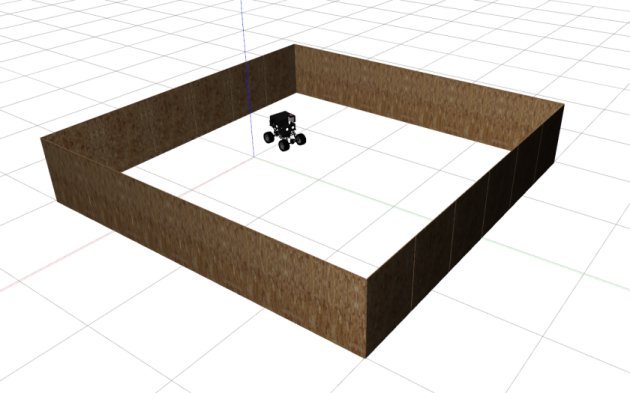
\includegraphics[width=\linewidth]{Chapters/Chapter5/Figures/simple_room.jpg}}
	\caption{Το περιβάλλον simple{\_}room που χρησιμοποιήθηκε για την εκτέλεση πειραμάτων  αξιολόγησης του κινηματικού μοντέλου στον προσομοιωτή Gazebo.}
	\label{fig:simple_room}
\end{figure}

\begin{figure}[!ht]
	\centering
	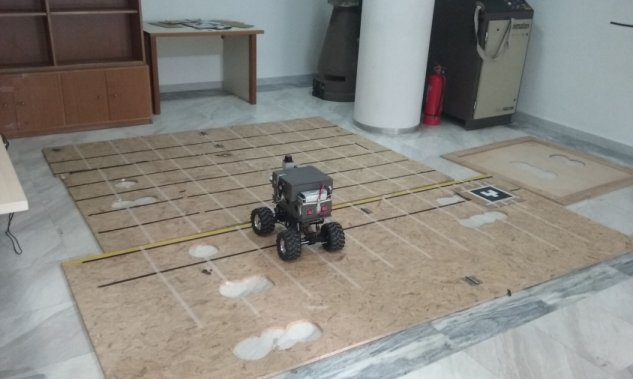
\includegraphics[width=\linewidth]{Chapters/Chapter5/Figures/pandora_arena.jpg}
	\caption{Η πίστα του εργαστηρίου της ομάδας P.A.N.D.O.R.A που χρησιμοποιήθηκε για την εκτέλεση πειραμάτων στο φυσικό ρομπότ για την αξιολόγηση του κινηματικού μοντέλου.}
	\label{fig:pandora_circuit}
\end{figure}

\bigskip
Για την εκτέλεση των πειραμάτων χρησιμοποιήθηκε το σύστημα χαρτογράφησης και εντοπισμού θέσης με τον αλγόριθμο CRSM-SLAM, ενώ ο έλεγχος του ρομπότ έγινε μέσω τηλεχειρισμού. Για την αξιολόγηση της συμπεριφοράς του ρομπότ, χρησιμοποιήθηκαν οι εντολές κίνησης που δόθηκαν στο ρομπότ, ως η επιθυμητή συμπεριφορά και η πραγματική τροχιά του ρομπότ, που εκδίδει ο αλγόριθμος CRSM-SLAM, ως η πραγματική συμπεριφορά.

\bigskip
Συνολικά, πραγματοποιήθηκαν δύο είδη πειραμάτων για την αξιολόγηση του κινηματικού μοντέλου και συγκεκριμένα για την αξιολόγηση της ακτίνας τροχιάς κατά την εκτέλεση κυκλικών τροχιών με αρνητική τετραδιεύθυνση και για την αξιολόγηση της πλευρικής γωνίας ολίσθησης κατά την εκτέλεση διαγώνιων ευθύγραμμων τροχιών με θετική τετραδιεύθυνση, όπως αυτά παρουσιάζονται στην συνέχεια.

\subsection{Τροχιές Αρνητικής Τετραδιεύθυνσης}
Για την αξιολόγηση της αρνητικής τετραδιεύθυνσης πραγματοποιήθηκε μία σειρά πειραμάτων, στην οποία, δόθηκαν εντολές στο ρομπότ για εκτέλεση κυκλικών τροχιών, για διάφορες δυνατές γωνίες στρέψης $\delta_f$, $\delta_r$ των μπροστινών και πίσω τροχών αντίστοιχα, για τις οποίες, έπειτα υπολογίστηκαν οι ιδανικές ακτίνες τροχιάς $R_{ideal}$ και οι πραγματικές $R_{sim}$ και $R_{real}$, προσομοίωσης και φυσικού ρομπότ αντίστοιχα, όπως αυτές παρουσιάζονται στον πίνακα \ref{tab:counter_steering_experiment} και στο σχήμα \ref{fig:counter_steering_experiment}. Με βάση τον πίνακα αυτόν, παρατηρείται μία μικρή απόκλιση των πραγματικών τροχιών που εκτελεί το ρομπότ σε σύγκριση με τις ιδανικές, κάτι που, παρόλα αυτά, είναι δικαιολογημένο, λόγω της μη ιδανικότητας του κινηματικού μοντέλου τετραδιεύθυνσης της ρομποτικής πλατφόρμας Monstertruck, όπως επίσης και την επιρροή φαινομένων τριβών και ολίσθησης στους τροχούς.
 
\begin{table}[!ht]
	\centering
	\captionof{table}{Αποτελέσματα πειράματος κινηματικού σε τροχιές αρνητικής τετραδιεύθυνσης.}
	\label{tab:counter_steering_experiment}
	\begin{tabular}{c | c |  c | c}
	 	\textbf{$\delta_f$}, \textbf{$-\delta_r$} & \textbf{$R_{ideal}$} & \textbf{$R_{sim}$} & \textbf{$R_{real}$} \\ \hline
	   %------------------------------------------------------------------------------
	   $0.4$ & $0.378$ & $0.377$ & $0.396$\\
 	   $0.32$ & $0.483$ & $0.519$ & $0.524$\\
  	   $0.24$ & $0.654$ & $0.722$ & $0.689$\\
   	   $0.16$ & $0.991$ & $1.023$ & $1.087$
   	\end{tabular}
\end{table}

\begin{figure}[!ht]
	\centering
	\subfloat[]{\frame{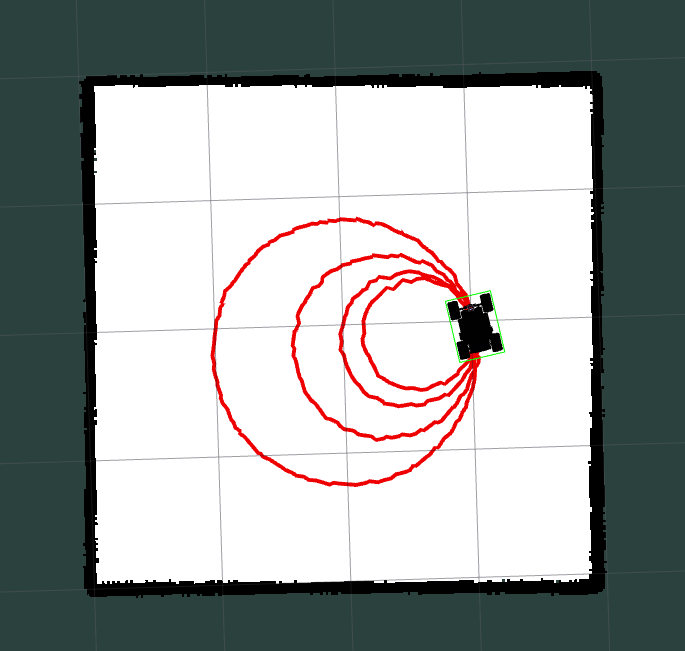
\includegraphics[height=7cm]{Chapters/Chapter5/Figures/counter_steering_experiment.png}}} \hspace{1cm}
	\subfloat[]{\frame{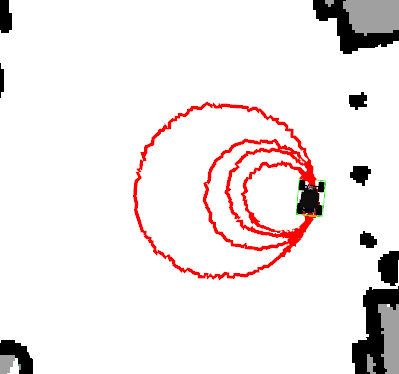
\includegraphics[height=7cm]{Chapters/Chapter5/Figures/counter_steering_experiment_real.png}}}
	\caption{Τροχιές που παράχθηκαν κατά τα πειράματα αξιολόγησης του κινηματικού μοντέλου σε τροχιές αρνητικής τετραδιεύθυνσης στα περιβάλλοντα (α') simple{\_}room και (β') πίστα της ομάδας P.A.N.D.O.R.A.}
	\label{fig:counter_steering_experiment}
\end{figure}


\subsection{Τροχιές Θετικής Τετραδιεύθυνσης}
Για την αξιολόγηση της θετικής τετραδιεύθυνσης πραγματοποιήθηκε μία σειρά πειραμάτων, στην οποία, δόθηκαν εντολές στο ρομπότ για εκτέλεση διαγώνιων τροχιών, για διάφορες δυνατές γωνίες στρέψης των τροχών $\delta_f$, $\delta_r$, τέτοιες ώστε $\delta_f = \delta_r$, ενώ, έπειτα, υπολογίστηκε η ιδανική γωνία πλευρικής ολίσθησης $\beta_{ideal}$, όπως επίσης και οι πραγματικές γωνίες πλευρικής ολίσθησης $\beta_{sim}$ και $\beta_{real}$ των πραγματικών τροχιών που εκτελέστηκαν από το ρομπότ σε επίπεδο προσομοίωσης και επίπεδο φυσικού ρομπότ αντίστοιχα και οι οποίες παρουσιάζονται στον πίνακα \ref{tab:crab_steering_experiment} και στο σχήμα \ref{fig:crab_steering_experiment}. Παρατηρείται, γενικά, πολύ μικρό έως αμελητέο σφάλμα της πραγματικής συμπεριφοράς του ρομπότ σε σύγκριση με την ιδανική και επομένως, αυτή, κρίνεται πλήρως αποδεκτή.

\bigskip 
\begin{table}[!ht]
	\centering
	\captionof{table}{Αποτελέσματα πειράματος κινηματικού σε τροχιές θετικής τετραδιεύθυνσης.}
	\label{tab:crab_steering_experiment}
	\begin{tabular}{c | c |  c | c}
	 	\textbf{$\delta_f$, $\delta_r$} & \textbf{$\beta_{ideal}$} & \textbf{$\beta_{sim}$} & \textbf{$\beta_{real}$} \\ \hline
	   %------------------------------------------------------------------------------
	   $0.4$ & $0.4$ & $0.398$ & $0.427$\\
 	   $0.32$ & $0.32$ & $0.326$ & $0.338$\\
  	   $0.24$ & $0.24$ & $0.232$ & $0.246$\\
   	   $0.16$ & $0.16$ & $0.151$ & $0.139$\\
   	\end{tabular}
\end{table}

\begin{figure}[!ht]
	\centering
	\subfloat[]{\frame{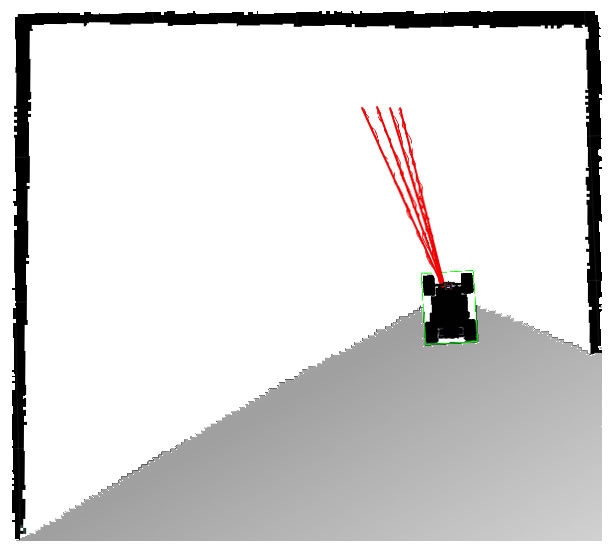
\includegraphics[height=6.5cm]{Chapters/Chapter5/Figures/crab_steering_experiment.png}}} \hspace{0.75cm}
	\subfloat[]{\frame{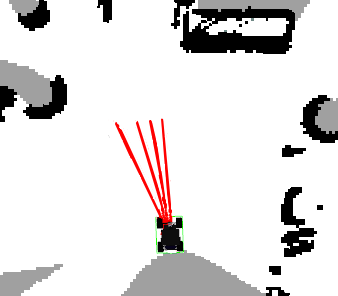
\includegraphics[height=6.5cm]{Chapters/Chapter5/Figures/crab_steering_experiment_real.png}}}
	\caption{Τροχιές που παράχθηκαν κατά τα πειράματα αξιολόγησης του κινηματικού μοντέλου σε τροχιές θετικής τετραδιεύθυνσης στα περιβάλλοντα (α´) simple{\_}room και (β') πίστα της ομάδας P.A.N.D.O.R.A.}
	\label{fig:crab_steering_experiment}
\end{figure}


%----------------------------------------------------------------------------------------
%	SECTION 2: SLAM Experiments
%----------------------------------------------------------------------------------------
\section{Πειράματα Χαρτογράφησης} \label{sec:slam_experiments}
Στην παρούσα ενότητα γίνεται μία αξιολόγηση των συστημάτων χαρτογράφησης και υπολογισμού θέσης, όπως αυτά παρουσιάσθηκαν στην ενότητα \ref{ssec:slam_components}, μέσω σύγκρισης των δύο επιμέρους συστημάτων, αλλά και μέσω σύγκρισης με τον πραγματικό χάρτη, εφόσον αυτός παρέχεται. Τα πειράματα πραγματοποιήθηκαν στον 2D προσομοιωτή STDR, στον 3D προσομοιωτή Gazebo, αλλά και στο φυσικό ρομπότ, με χρήση των συστημάτων χαρτογράφησης και εντοπισμού θέσης των αλγορίθμων CRSM-SLAM και Gmapping.

\bigskip
Για την χαρτογράφηση του περιβάλλοντος, η ρομποτική πλατφόρμα Monstertruck χρησιμοποιεί ως βασικό εργαλείο τον σαρωτή λέιζερ Hokuyo URG-04LX, ο οποίος έχει εμβέλεια $4m$ και επομένως τα περιβάλλοντα των πειραμάτων επιλέχθηκαν αναλόγως. Συγκεκριμένα, επιλέχθηκαν περιβάλλοντα με εσωτερικούς κλειστούς χώρους, με αρκετά στενούς διαδρόμους και δωμάτια με επαρκή ποικιλομορφία για την όσο το δυνατόν πιο αξιόπιστη χαρτογράφηση. Επίσης, λόγω της περιορισμένης υπολογιστικής ισχύος του υπολογιστή ODROID-XU4, της ρομποτικής πλατφόρμας Monstertruck, επιλέχθηκε ανάλυση χαρτογράφησης ίση με $0.04m$ και γενικότερα ειδική παραμετροποίηση των αλγορίθμων SLAM, έτσι ώστε να επιτευχθεί ταυτόχρονα αύξηση της συχνότητας ανανέωσης του χάρτη και μείωση του υπολογιστικού φόρτου, με επίδραση, παρόλα αυτά, στην ποιότητα του.

\subsection{Χαρτογράφηση στον 2D Προσομοιωτή STDR} \label{ssec:stdr_slam}
%------------------------------------------------%
Για τα πειράματα στον προσομοιωτή STDR, επιλέχθηκε ο χάρτης \textit{robocup} που παρέχεται από τον προσομοιωτή, λόγω της πολυπλοκότητας του και της ομοιότητας του με τα περιβάλλοντα για τα οποία προορίζεται η ρομποτική πλατφόρμα Monstertruck. Παρόλα αυτά, μετά από αρχικά πειράματα, διαπιστώθηκε ότι ο χάρτης είχε κάποιους μεγάλους ομοιόμορφους διαδρόμους που δημιουργούσαν πρόβλημα στην χαρτογράφηση, με τον αλγόριθμο CRSM-SLAM, λόγω αδυναμίας εντοπισμού της ακριβής θέσης, εξαιτίας του περιορισμένου εύρους του σαρωτή λέιζερ και άρα της εσφαλμένης αντιστοίχισης σκαναρισμάτων. Γι αυτό το λόγο, κρίθηκε σκόπιμο να μειωθεί η ανάλυση του χάρτη από $0.03$ σε $0.02$ με στόχο την μείωση της κλίμακας του. Στο σχήμα \ref{fig:stdr_robocup} παρουσιάζεται ο χάρτης robocup και οι αντίστοιχοι χάρτες που κατασκεύασαν οι αλγόριθμοι CRSM-SLAM και Gmapping.

\begin{figure}[!ht]
	\centering
	\subfloat[Ground Truth.]{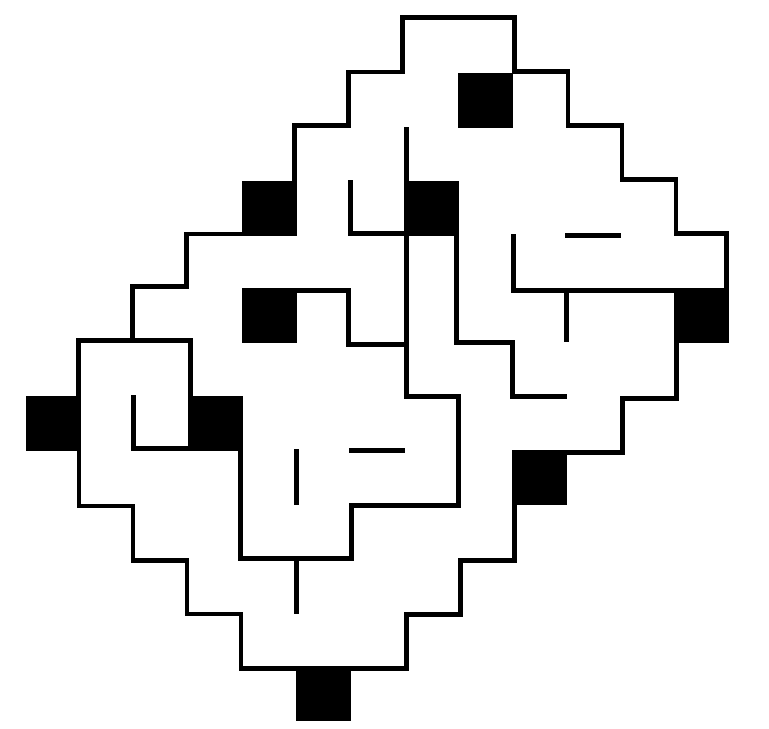
\includegraphics[width=0.31\linewidth, height=5cm]{Chapters/Chapter5/Figures/stdr_robocup_ground_truth.png}}
	\subfloat[CRSM-SLAM]{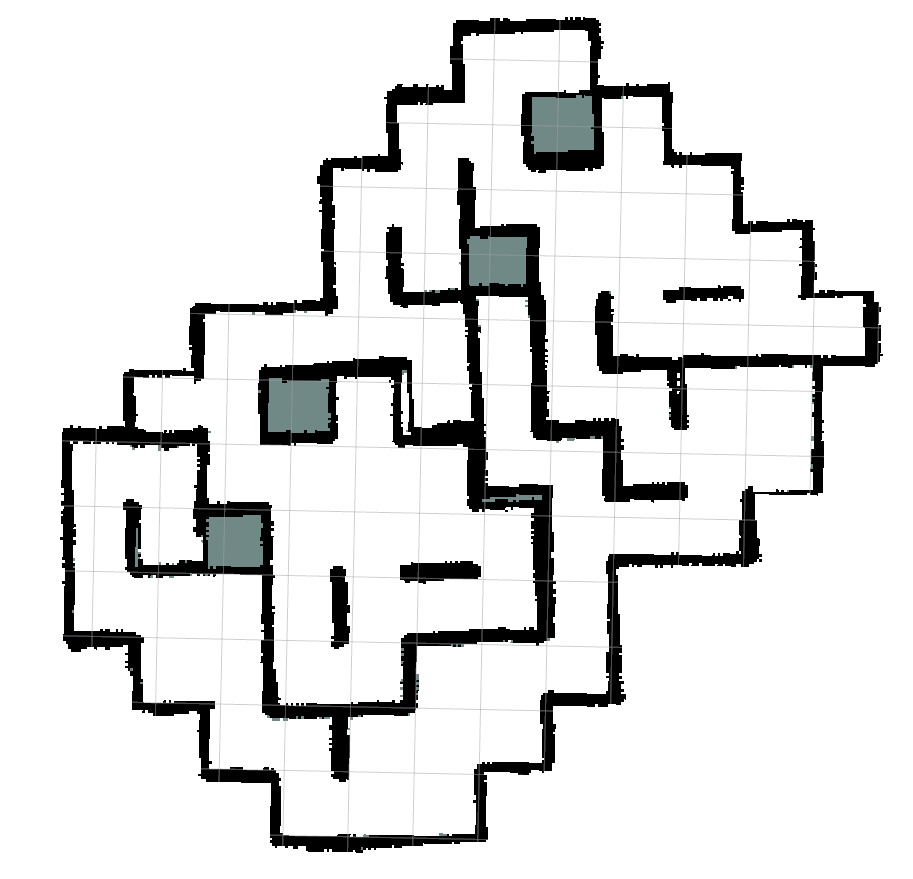
\includegraphics[width=0.31\linewidth, height=5cm]{Chapters/Chapter5/Figures/stdr_robocup_crsm.png}}
	\subfloat[Gmapping]{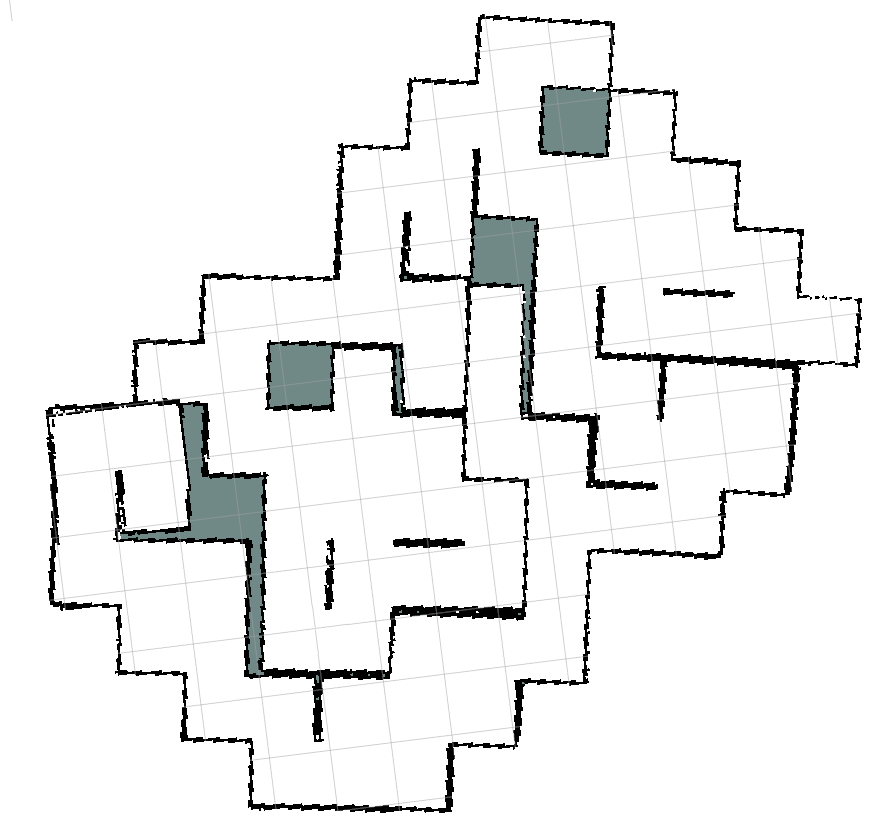
\includegraphics[width=0.31\linewidth, height=5cm]{Chapters/Chapter5/Figures/stdr_robocup_gmapping.png}}
	\caption{Χάρτες του περιβάλλοντος robocup.}
	\label{fig:stdr_robocup}
\end{figure}

\bigskip
Βάσει του σχήματος \ref{fig:stdr_robocup}, παρατηρείται, ότι τα δύο συστήματα χαρτογράφησης που εξετάστηκαν, παράγουν μία αναπαράσταση του περιβάλλοντος robocup, με αρκετές ατέλειες, αλλά χωρίς να υπάρχει κάποιο εξαιρετικά μεγάλο σφάλμα που να επιδρά σημαντικά στην ακεραιότητα του χάρτη και επομένως κρίνονται ικανοποιητικά για τα πλαίσια της παρούσας εργασίας.

\subsection{Χαρτογράφηση στον 3D προσομοιωτή Gazebo} \label{ssec:gazebo_slam}
%--------------------------------------------------%
Για τα πειράματα χαρτογράφησης στον προσομοιωτή Gazebo, επιλέχθηκε ο χάρτης της αρένας του διαγωνισμού RoboCup Rescue 2013, σε δύο εκδοχές, με ομαλό και ανώμαλο έδαφος για την εξέταση της συμπεριφοράς του συστήματος, υπό όλες τις δυνατές συνθήκες για τις οποίες προορίζεται να λειτουργήσει αυτό.

\bigskip
Για την διεξαγωγή των πειραμάτων, το ρομπότ τέθηκε σε λειτουργία αυτόματης εξερεύνησης χωρίς κάποια χειροκίνητη παρέμβαση, για την κάλυψη όλης της αρένας για τις περιπτώσεις ομαλού και ανώμαλου εδάφους, με στόχο την πλήρη χαρτογράφηση αυτών, μέσω των αλγορίθμων CRSM-SLAM και Gmapping.

\subsubsection{Χαρτογράφηση της Αρένας RoboCup Rescue 2013 με Ομαλό Έδαφος}
Για την χαρτογράφηση, σε ομαλό έδαφος, η αρένα RoboCup Rescue 2013 προσαρμόστηκε κατάλληλα για να επιτρέπει την πλήρη προσπέλαση της από το ρομπότ, μέσω της αφαίρεσης ανυψωμένων τμημάτων, όπως ράμπες, σκάλες κοκ. Στο σχήμα \ref{fig:robocup_2013_arena_flat} παρουσιάζεται η προσαρμοσμένη αρένα RoboCup Rescue 2013, με ομαλό έδαφος, όπως επίσης και οι αντίστοιχοι χάρτες που κατασκευάστηκαν από τους αλγορίθμους CRSM-SLAM και Gmapping.

\bigskip
Συγκρίνοντας, τους παραγόμενους χάρτες με το πραγματικό περιβάλλον παρατηρούνται κάποια σφάλματα συστροφής μεταξύ των οριζόντιων διαδρόμων της αρένας, που παρόλα αυτά, δεν επιδρούν σημαντικά στην ακεραιότητα του χάρτη. Τα δύο συστήματα χαρτογράφησης κατασκεύασαν επαρκείς αναπαραστάσεις της αρένας, με ελαφρώς καλύτερη αυτή του αλγορίθμου Gmapping, εις βάρος, παρόλα αυτά των απαιτήσεων αυτού σε υπολογιστική ισχύ και πλήθος δεδομένων. 

\subsubsection{Χαρτογράφηση της Αρένας RoboCup Rescue 2013 με Ανώμαλο Έδαφος}
Για την περίπτωση της αρένας με ανώμαλο έδαφος, χρησιμοποιήθηκε αρχικά η ακέραιη εκδοχή της αρένας RoboCup Rescue 2013, αλλά παρατηρήθηκε ότι περιείχε τμήματα τα οποία δεν ήταν δυνατόν να γίνουν αντιληπτά, ενώ παράλληλα δεν ήταν ούτε προσπελάσιμα από το ρομπότ. Επομένως, κρίθηκε σκόπιμο, η εν λόγω αρένα να προσαρμοστεί, ούτως ώστε να αφαιρεθούν τα τμήματα αυτά. Συγκεκριμένα, αφαιρέθηκαν από την αρένα τα ακόλουθα τμήματα, όπως αυτά παρουσιάζονται ακολούθως και στο σχήμα \ref{fig:removed_parts_from_robocup_arena}:

\begin{itemize}
	\item Μία σκάλα, η οποία είχε κενό μεταξύ των σκαλοπατιών, με αποτέλεσμα να περνάνε διαμέσου αυτής οι ακτίνες του σαρωτή λέιζερ και άρα αυτήν να γίνεται αντιληπτή εσφαλμένα ως ελεύθερος χώρος.
	\item Μία ράμπα μεγάλης κλίσης, της οποίας το κατώτερο τμήμα δεν αναγνωριζόταν ως εμπόδιο, με κίνδυνο σύγκρουσης με το ρομπότ.
	\item Ένα σύνολο τμημάτων με υψηλά και άνισα κομμάτια που προεξείχαν σε αρκετά χαμηλό ύψος, ώστε να μην χτυπάνε οι ακτίνες του λέιζερ σ' αυτά, αλλά παράλληλα αρκετά ψηλά, ώστε να προκαλούν την προσκόλληση ή ακόμα και ανατροπή του ρομπότ.
\end{itemize}

\begin{figure}[!ht]
	\subfloat[Σκάλα.]{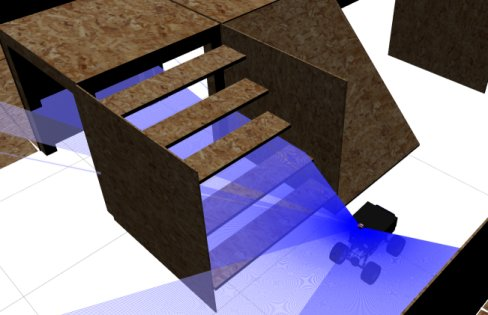
\includegraphics[width=0.32\linewidth, height=3.5cm]{Chapters/Chapter5/Figures/staircase.jpg}}
	\hspace{0.01\linewidth}
	\subfloat[Ράμπα μεγάλης κλίσης.]{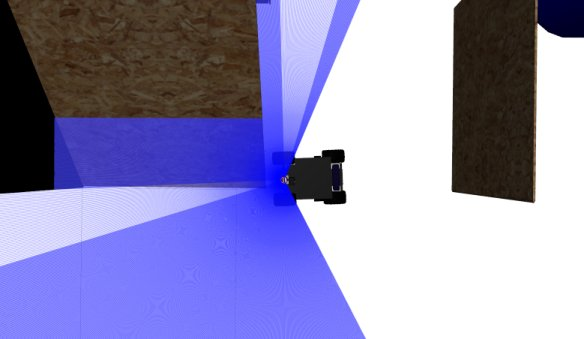
\includegraphics[width=0.32\linewidth, height=3.5cm]{Chapters/Chapter5/Figures/big_ramp.jpg}}
	\hspace{0.01\linewidth}
	\subfloat[Μη αντιλήψιμα και μη προσπελάσιμα εμπόδια.]{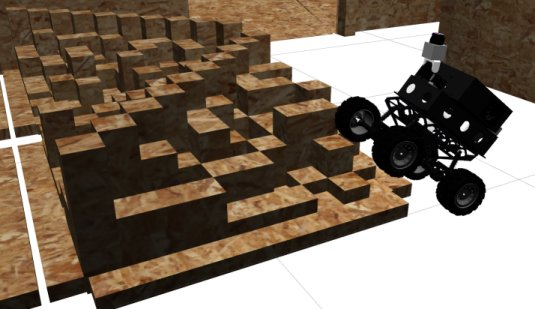
\includegraphics[width=0.32\linewidth, height=3.5cm]{Chapters/Chapter5/Figures/stepfield.jpg}}
	\caption{Τα τμήματα που αφαιρέθηκαν από την αρένα με το ανώμαλο έδαφος, λόγω της αδυναμίας εντοπισμού και προσπελασιμότητας από την ρομποτική πλατφόρμα Monstertruck.}
	\label{fig:removed_parts_from_robocup_arena}
\end{figure}

\bigskip
Αφού αφαιρεθούν τα παραπάνω εμπόδια από τον χάρτη, το ανώμαλο έδαφος προσεγγίζεται, πλέον, με ξύλινες ράμπες με κλίση περίπου $15^o$. Η αξιόπιστη χαρτογράφηση περιβάλλοντος, αυτού του τύπου, καθίσταται δυνατή από την αντιστάθμιση κλίσης roll και pitch του σαρωτή λέιζερ, μέσω του μηχανισμού σταθεροποίησης αυτού, σε συνδυασμό με την πυξίδα που παρέχει τις μετρήσεις των κλίσεων roll και pitch του ρομπότ. Στα σχήματα \ref{fig:robocup_2013_arena} που ακολουθούν, παρουσιάζεται η προσαρμοσμένη αρένα και οι αντίστοιχοι χάρτες.

\bigskip
Οι χάρτες που κατασκεύασαν τα δύο συστήματα SLAM για την αρένα με το ανώμαλο έδαφος παρουσιάζουν εξαιρετικά μεγάλη ομοιότητα με τους αντίστοιχους χάρτες της αρένας με το ομαλό έδαφος, γεγονός που αποδεικνύει την ευρωστία του συστήματος σε όλες τις πιθανές συνθήκες λειτουργίας.

\subsection{Χαρτογράφηση σε Πραγματικό Περιβάλλον με τη Ρομποτική Πλατφόρμα Monstertruck}
%---------------------------------%
Πέρα από τα πειράματα χαρτογράφησης σε επίπεδο προσομοίωσης, αντίστοιχα πειράματα πραγματοποιήθηκαν για τη φυσική ρομποτική πλατφόρμα Monstertruck. Για την εκτέλεση των πειραμάτων με το φυσικό ρομπότ, επιλέχθηκε ο χώρος του {Εργαστηρίου Αρχιτεκτονικής και Υπολογιστών}, του τμήματος Ηλεκτρολόγων Μηχανικών και Μηχανικών Υπολογιστών, του Αριστοτελείου Πανεπιστημίου Θεσσαλονίκης. Ο χώρος αυτός αποτελεί ένα δωμάτιο με τρεις σειρές γραφείων υπολογιστών με καρέκλες και περιλαμβάνει εξ ολοκλήρου ομαλό έδαφος. Για την αύξηση της πολυπλοκότητας του εν λόγω χώρου, παρόλα αυτά, προστέθηκαν και ξύλινες ράμπες για την επαλήθευση των αποτελεσμάτων που λήφθηκαν κατά την προσομοίωση, υπό όλες τις δυνατές συνθήκες.  Στο σχήμα \ref{fig:csal} παρουσιάζεται ο χώρος του εργαστηρίου, όπως επίσης και οι αντίστοιχοι χάρτες που παράχθηκαν, βάσει αυτού, μέσω των αλγορίθμων CRSM-SLAM και Gmapping.

\begin{figure}[!ht]
	\centering
	\subfloat[Εργαστήριο Αρχιτεκτονικής Υπολογιστών.]{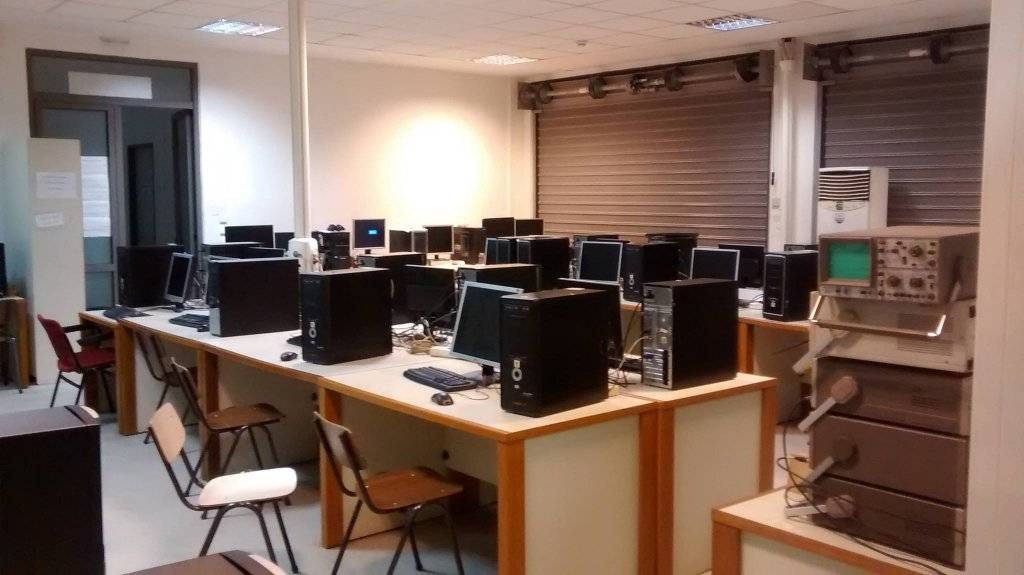
\includegraphics[width=0.7\linewidth]{Chapters/Chapter5/Figures/csal.jpg}}\\
	\subfloat[Χάρτης μέσω CRSM-SLAM.]{\frame{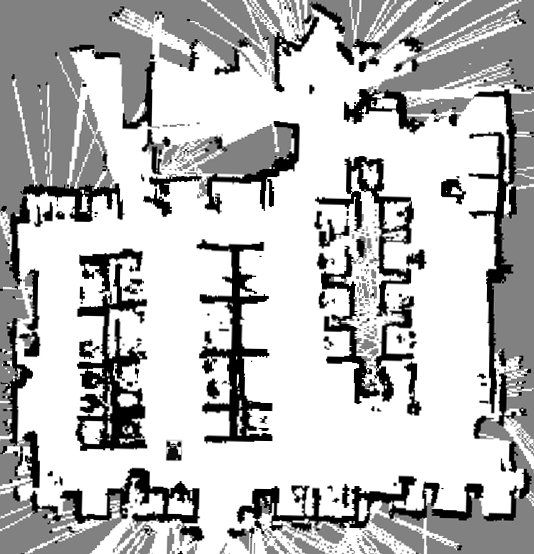
\includegraphics[height=7.5cm]{Chapters/Chapter5/Figures/csal_crsm_map.jpg}}}
	\hspace{1.0cm}
	\subfloat[Χάρτης μέσω Gmapping.]{\frame{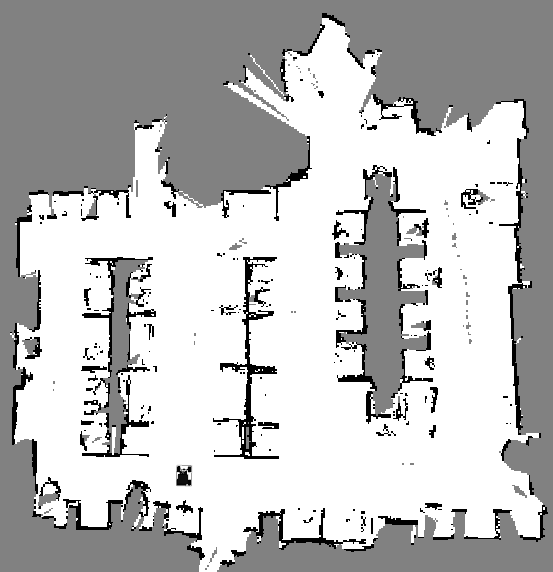
\includegraphics[height=7.5cm]{Chapters/Chapter5/Figures/csal_gmapping_map.png}}}
	\caption{Εργαστήριο Αρχιτεκτονικής Υπολογιστών, Τμήματος ΗΜΜΥ, ΑΠΘ και οι αντίστοιχοι χάρτες που κατασκευάστηκαν.}
	\label{fig:csal}
\end{figure}

\begin{figure}[!ht]
	\centering
	\subfloat[Αρένα RoboCup Rescue 2013 με ομαλό έδαφος.]{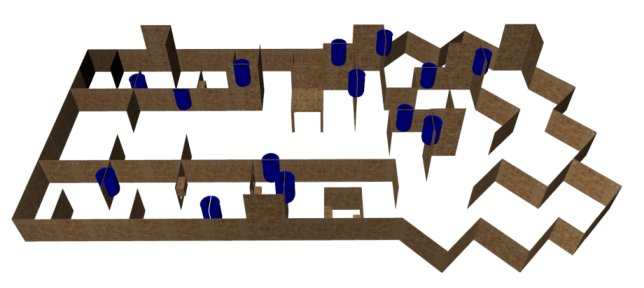
\includegraphics[height=6.5cm]{Chapters/Chapter5/Figures/robocup_2013_arena_flat.jpg}}\\
	\subfloat[Χάρτης μέσω CRSM-SLAM.]{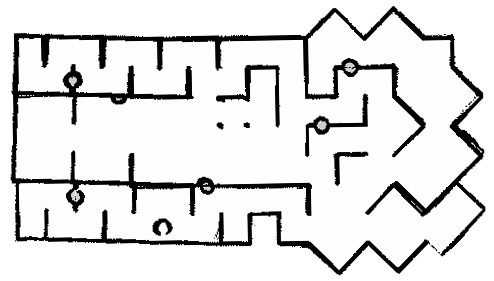
\includegraphics[height=7cm]{Chapters/Chapter5/Figures/robocup_arena_flat_crsm_map.png}}\\
	\subfloat[Χάρτης μέσω Gmapping.]{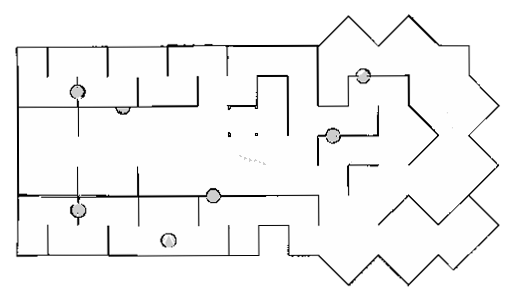
\includegraphics[height=7cm]{Chapters/Chapter5/Figures/robocup_arena_flat_gmapping_map.png}}
	\caption{Η αρένα του διαγωνισμού RoboCup Rescue 2013 με ομαλό έδαφος και οι αντίστοιχοι παραγόμενοι χάρτες.}
	\label{fig:robocup_2013_arena_flat}
\end{figure}

\begin{figure}[!ht]
	\centering
	\subfloat[Αρένα RoboCup Rescue 2013 με ανώμαλο έδαφος.]{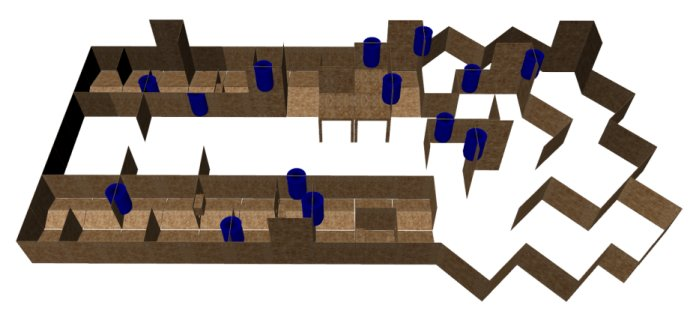
\includegraphics[height=6.5cm]{Chapters/Chapter5/Figures/robocup_2013_arena.jpg}}\\
	\subfloat[Χάρτης μέσω CRSM-SLAM.]{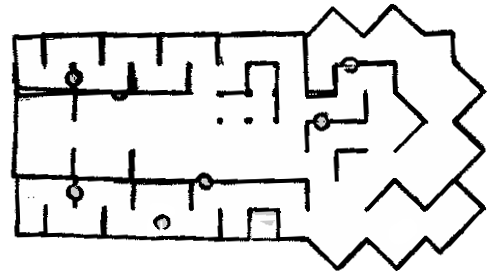
\includegraphics[height=7cm]{Chapters/Chapter5/Figures/robocup_arena_crsm_map.png}}\\
	\subfloat[Χάρτης μέσω Gmapping.]{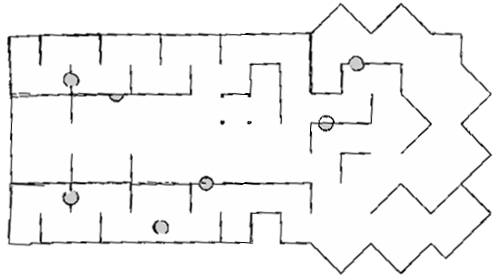
\includegraphics[height=7cm]{Chapters/Chapter5/Figures/robocup_arena_gmapping_map.png}}
	\caption{Η αρένα του διαγωνισμού RoboCup Rescue 2013 με ανώμαλο έδαφος και οι αντίστοιχοι παραγόμενοι χάρτες.}
	\label{fig:robocup_2013_arena}
\end{figure}

\FloatBarrier

%----------------------------------------------------------------------------------------
%	SECTION 3: Navigation Experiments
%----------------------------------------------------------------------------------------

\newpage
\section{Πειράματα Αυτόνομης Πλοήγησης} \label{sec:navigation_experiments}
Στην παρούσα ενότητα παρουσιάζονται πειράματα σχετικά με τα επιμέρους τμήματα των συστημάτων αυτόνομης πλοήγησης της ρομποτικής πλατφόρμας Monstertruck, όπως επίσης και μία σύγκριση μεταξύ αυτών, ενώ τελικά παρουσιάζεται και η συνολική συμπεριφορά των δύο συστημάτων. Συγκεκριμένα, παρουσιάζεται η συμπεριφορά των αλγορίθμων κατασκευής μονοπατιών, του αλγορίθμου παραμόρφωσης μονοπατιού Reeds-Shepp Band, ο αλγόριθμος διάσχισης μονοπατιού που βασίζεται σε ασαφή λογική, ενώ τέλος γίνεται και μία σύγκριση μεταξύ του συστήματος αυτόνομης πλοήγησης με δυναμική παραμόρφωση μονοπατιού και του συστήματος αυτόνομης πλοήγησης με δυναμική ανακατασκευή μονοπατιού.

\subsection{Κατασκευή Μονοπατιών} \label{ssec:path_planning_experiments}
Τα πειράματα κατασκευής μονοπατιού πραγματοποιήθηκαν στον 2D προσομοιωτή STDR, χωρίς την χρήση κάποιου αλγορίθμου SLAM, αλλά χρησιμοποιώντας το ground truth του χάρτη του περιβάλλοντος και την τέλεια οδομετρία που παρέχει ο προσομοιωτής, για εντοπισμό της θέσης του ρομπότ. Για την διεξαγωγή των πειραμάτων, επιλέχθηκε το περιβάλλον sparse{\_}obstaceles που παρέχει ο προσομοιωτής STDR και το οποίο παρουσιάζεται στο σχήμα \ref{fig:sparse_obstacles}.

\begin{figure}[!ht]
	\centering
	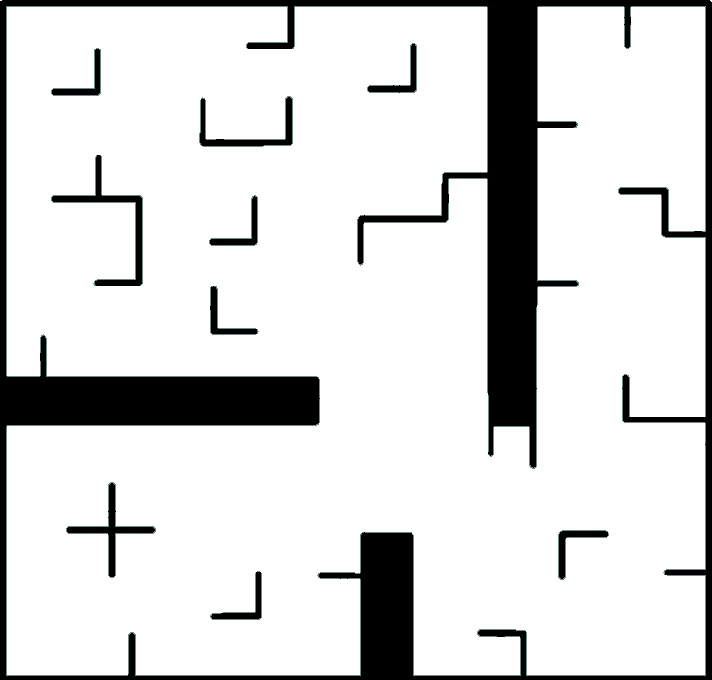
\includegraphics[width=0.4\linewidth]{Chapters/Chapter5/Figures/sparse_obstacles.png}
	\caption{Το περιβάλλον sparse{\_}obstacles του προσομοιωτή\\ STDR, που χρησιμοποιήθηκε για τα πειράματα\\κατασκευής μονοπατιού.}
	\label{fig:sparse_obstacles}
\end{figure}

\bigskip
Για την περίπτωση των αλγορίθμων Dijkstra και A* που υλοποιεί το plugin global{\_}planner, ορίζονται δύο μετρικές αξιολόγησης, όπου, η πρώτη μετρική είναι ο χρόνος $T$ που απαιτεί ο αλγόριθμος για την κατασκευή του μονοπατιού, ενώ η δεύτερη μετρική είναι το συνολικό μήκος $s$ του μονοπατιού. Παράλληλα, μπορεί να γίνει και μία ποιοτική αξιολόγηση των αλγορίθμων Dijkstra και A*, βάσει του καλυπτόμενου χώρου αναζήτησης.

\bigskip
Στην περίπτωση των αλγορίθμων ARA* και AD* που υλοποιεί το plugin sbpl{\_}global{\_}planner, δεν είναι δυνατή η χρήση των ίδιων μετρικών με τους Dijkstra και A*, μιας και οι αλγόριθμοι αυτοί, χρησιμοποιούν σταθερό χρόνο $T$ για την κατασκευή ενός άκρως μη βέλτιστου μονοπατιού, ενώ παράλληλα συνεχίζουν την διαρκή βελτιστοποίηση αυτού, μειώνοντας σταδιακά τον παράγοντα διαστολής $\epsilon$ και βελτιστοποιώντας το μονοπάτι αυτό για τον τρέχοντα παράγοντα $\epsilon$ σε διάστημα $T$. Επομένως, ορίζονται δύο νέες μετρικές, το μήκος $s_{init}$ του αρχικού μη βέλτιστου μονοπατιού και το τελικό μήκος $s_{final}$ του τελικού μονοπατιού. Επίσης, αναφέρεται ότι επιλέχθηκε, χρόνος κατασκευής μονοπατιού $T=0.1s$ και αρχικός παράγοντας διαστολής $\epsilon_{init}=3$. 

\bigskip
Για την εξέταση και σύγκριση της συμπεριφοράς των παραπάνω αλγορίθμων, ορίστηκαν πέντε πόζες $p_i$, $i=1,...,4$, του περιβάλλοντος sparse{\_}obstacles, ως στόχοι, για την κατασκευή μονοπατιών, από την αρχική πόζα $p_0 = (1.5, 1.5, 90^o)$ του ρομπότ, όπως αυτές παρουσιάζονται στον πίνακα \ref{tab:path_planning_target_poses}.

\bigskip 
\begin{table}[!ht]
	\centering
	\captionof{table}{Οι στόχοι των πειραμάτων κατασκευής μονοπατιών\\ στο περιβάλλον sparse{\_}obstacles.}
	\label{tab:path_planning_target_poses}
	\begin{tabular}{| c | c  c  c |} \hline
	 	& $\mathbf{x[m]}$ & $\mathbf{y[m]}$ & $\mathbf{\theta[μοίρες]}$  \\ \hline
	   %------------------------------------------------------------------------------
 	   $p_1$ & $7$ & $2$ & $0$\\ 
  	   $p_2$ & $10$ & $1$ & $0$\\ 
   	   $p_3$ & $14$ & $11$ & $0$\\ 
		$p_4$ & $1.5$ & $11$ & $45^o$\\ \hline
   	\end{tabular}
\end{table}

Στην συνέχεια παρουσιάζονται στα σχήματα \ref{fig:dijkstra_experiments}-\ref{fig:adstar_experiments} τα τελικά μονοπάτια που κατασκευάζουν οι αλγόριθμοι κατασκευής μονοπατιών για την μετάβαση από την πόζα $p_0$ στις πόζες $p_i$, $i=1,...,4$, ενώ έπειτα, στον πίνακα \ref{tab:path_planning_experiments} με τα αποτελέσματα των μετρικών για τα εν λόγω μονοπάτια. Για τις περιπτώσεις των αλγορίθμων Dijkstra και A*, στα σχήματα \ref{fig:dijkstra_experiments}, \ref{fig:astar_experiments}, εικονίζεται, παράλληλα και η εξάπλωση του κάθε αλγορίθμου κατά την αναζήτηση του στόχου, με διακύμανση από μπλε έως κόκκινο βάσει της απόστασης από την αρχική θέση. Επιπλέον, στα σχήματα \ref{fig:arastar_successive_paths_experiment} και \ref{fig:adstar_successive_paths_experiment} παρουσιάζονται ενδεικτικές ακολουθίες βελτιστοποίησης μονοπατιού, μέσω των αλγορίθμων ARA* και AD*, για τυχαίο στόχο και για φθίνοντα παράγοντα διαστολής $\epsilon$ από $\epsilon_{init}=3$ έως $\epsilon_{final}=1$.

\begin{figure}[!ht]
	\centering
	\subfloat[$p_1$]{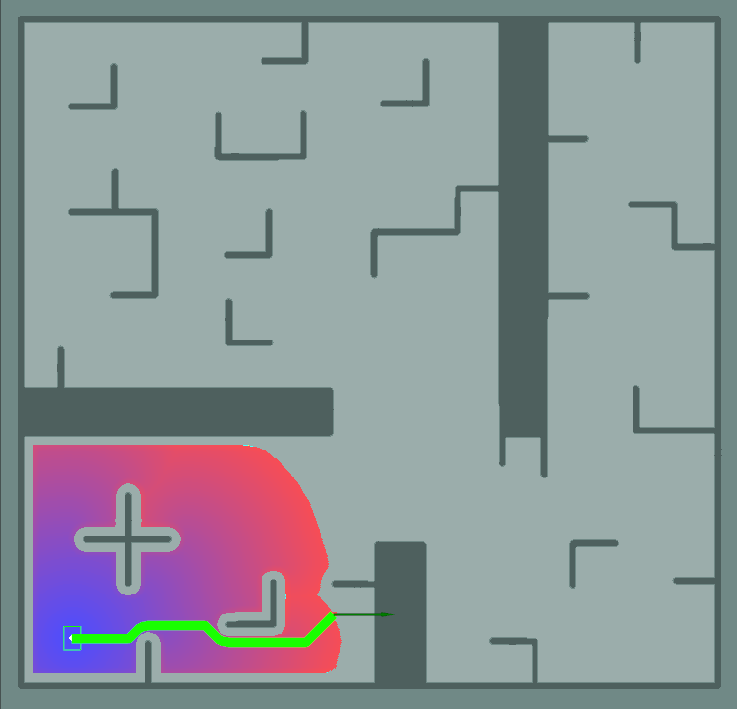
\includegraphics[width=0.24\linewidth]{Chapters/Chapter5/Figures/global_planner/so_dijkstra_p1.png}} \vspace{0.01\linewidth}
	\subfloat[$p_2$]{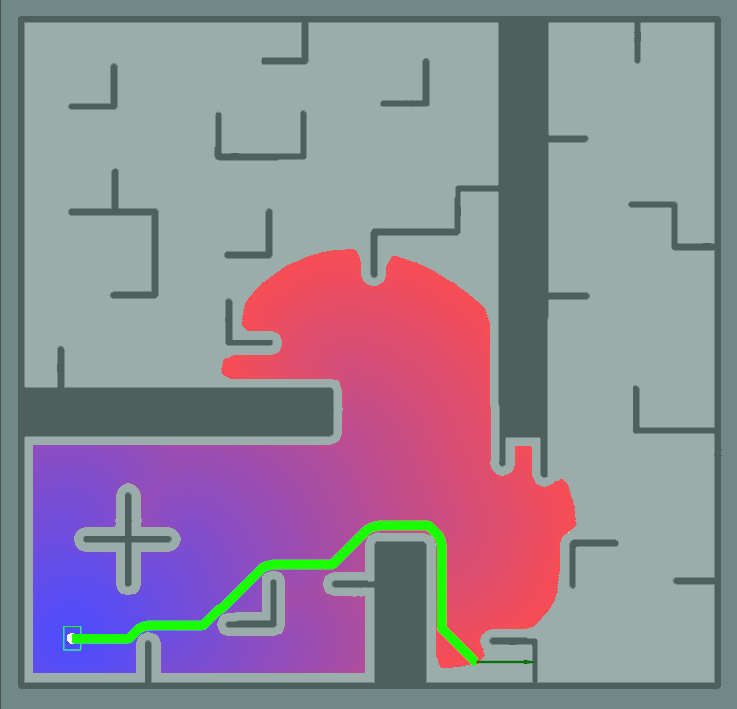
\includegraphics[width=0.24\linewidth]{Chapters/Chapter5/Figures/global_planner/so_dijkstra_p2.png}} \vspace{0.01\linewidth}
 	\subfloat[$p_3$]{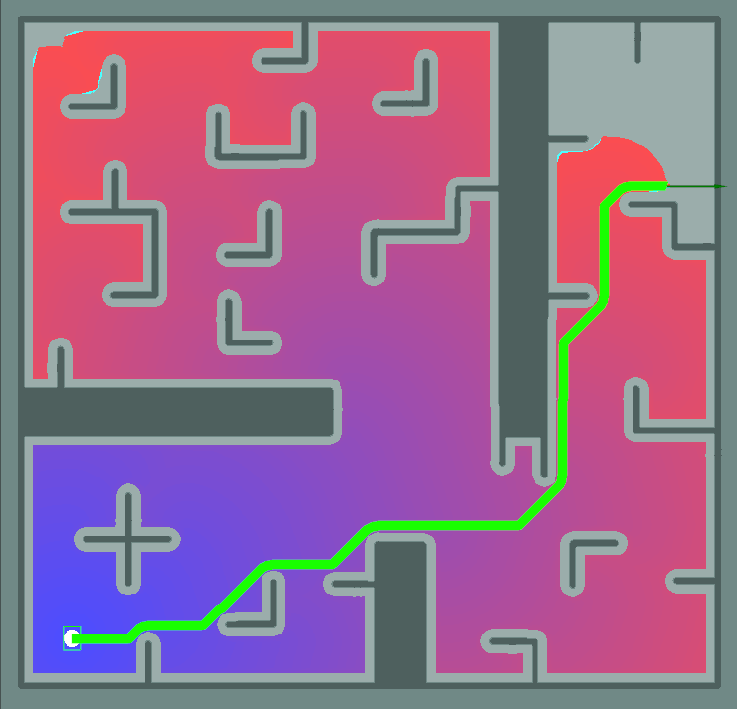
\includegraphics[width=0.24\linewidth]{Chapters/Chapter5/Figures/global_planner/so_dijkstra_p3.png}} \vspace{0.01\linewidth}
	\subfloat[$p_4$]{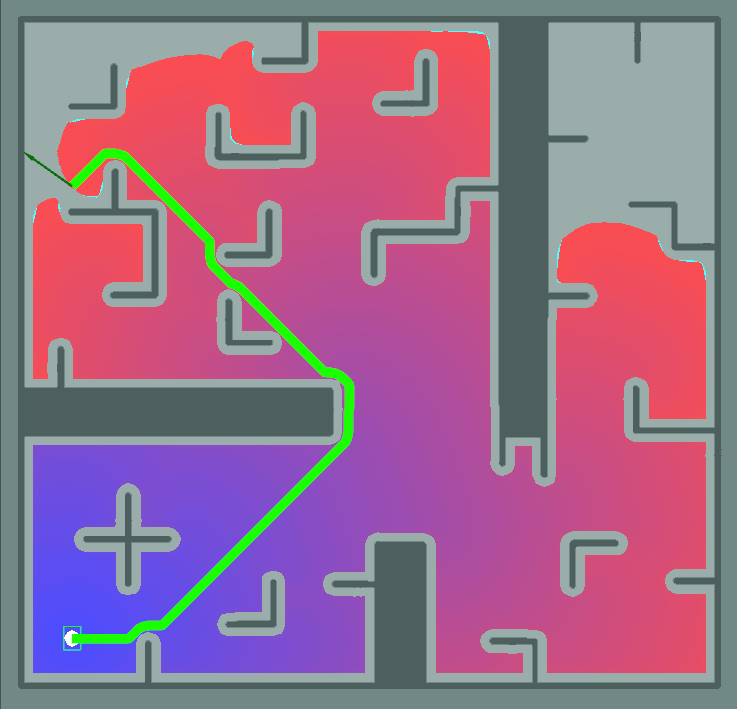
\includegraphics[width=0.24\linewidth]{Chapters/Chapter5/Figures/global_planner/so_dijkstra_p4.png}}
	\caption{Κατασκευή μονοπατιών με τον αλγόριθμο Dijkstra, για τις πόζες-στόχους $p_i$, $i=1,...,4$.}
	\label{fig:dijkstra_experiments}
\end{figure}

\begin{figure}[!ht]
	\centering
	\subfloat[$p_1$]{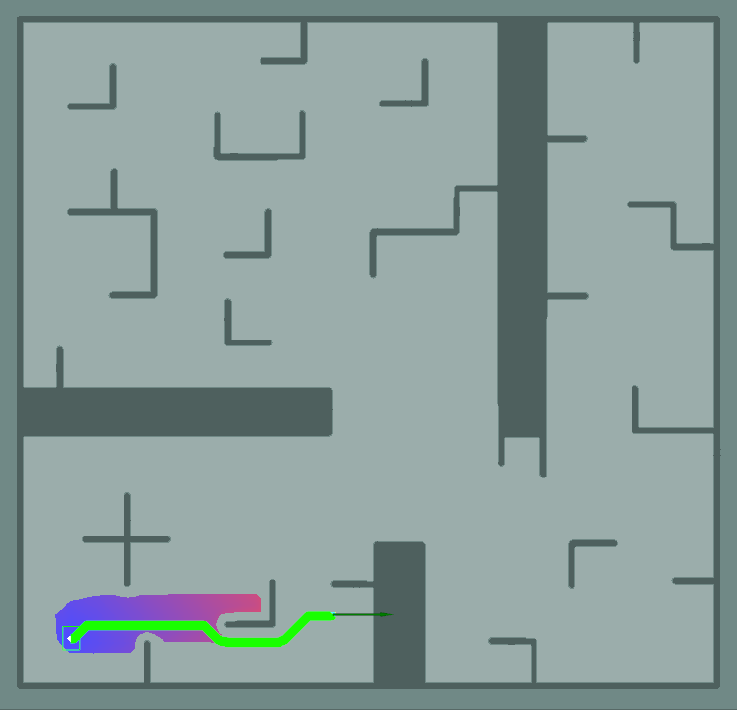
\includegraphics[width=0.24\linewidth]{Chapters/Chapter5/Figures/global_planner/so_astar_p1.png}} \vspace{0.01\linewidth}
	\subfloat[$p_2$]{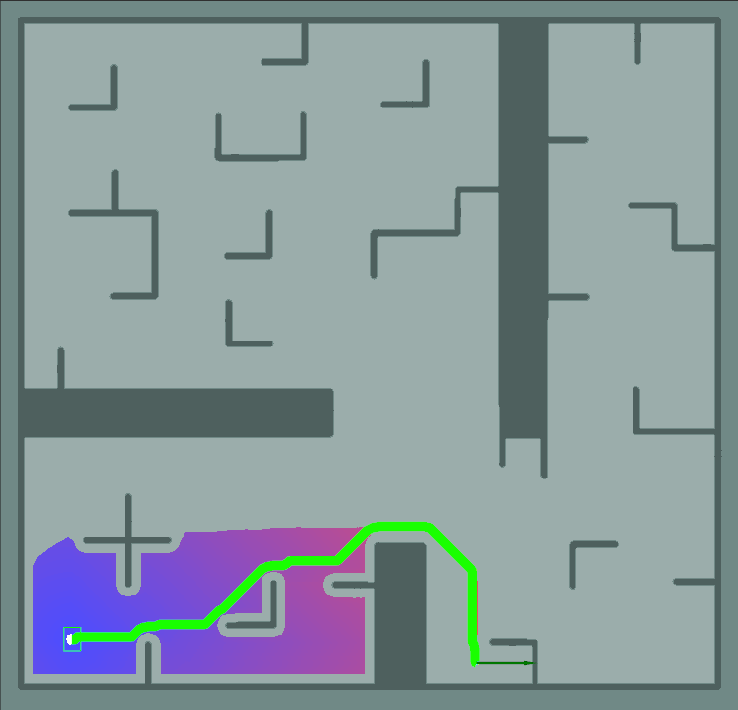
\includegraphics[width=0.24\linewidth]{Chapters/Chapter5/Figures/global_planner/so_astar_p2.png}} \vspace{0.01\linewidth}
 	\subfloat[$p_3$]{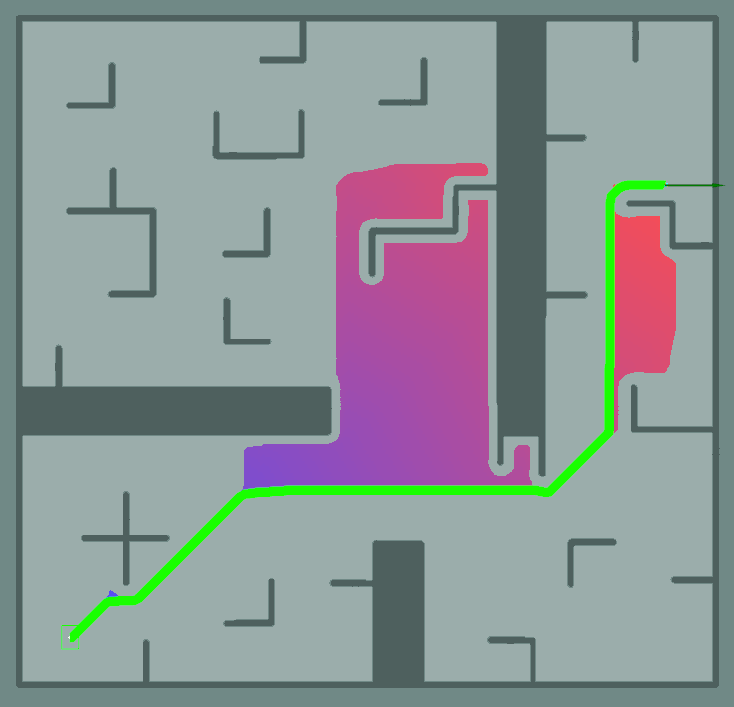
\includegraphics[width=0.24\linewidth]{Chapters/Chapter5/Figures/global_planner/so_astar_p3.png}} \vspace{0.01\linewidth}
	\subfloat[$p_4$]{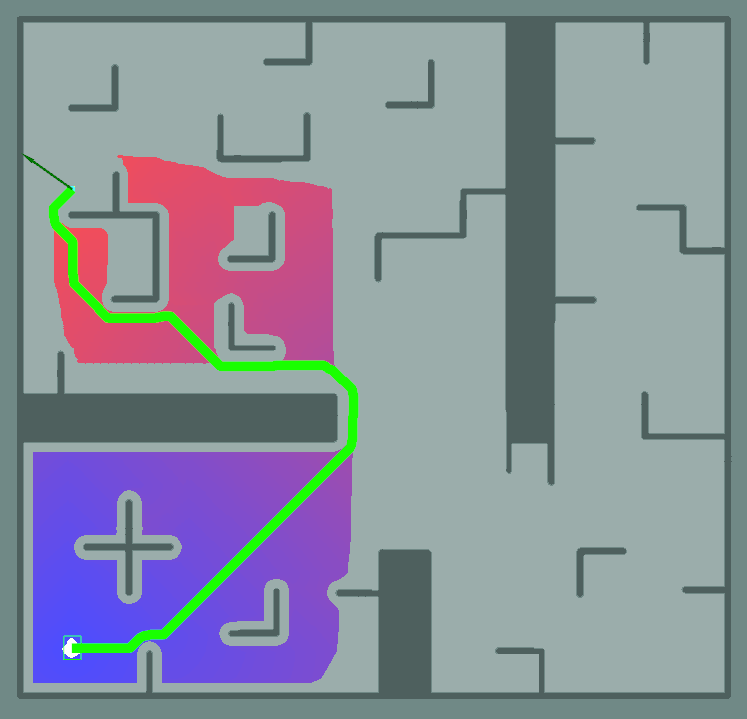
\includegraphics[width=0.24\linewidth]{Chapters/Chapter5/Figures/global_planner/so_astar_p4.png}}
	\caption{Κατασκευή μονοπατιών με τον αλγόριθμο A*, για τις πόζες-στόχους $p_i$, $i=1,...,4$.}
	\label{fig:astar_experiments}
\end{figure}

\begin{figure}[!ht]
	\centering
	\subfloat[$p_1$]{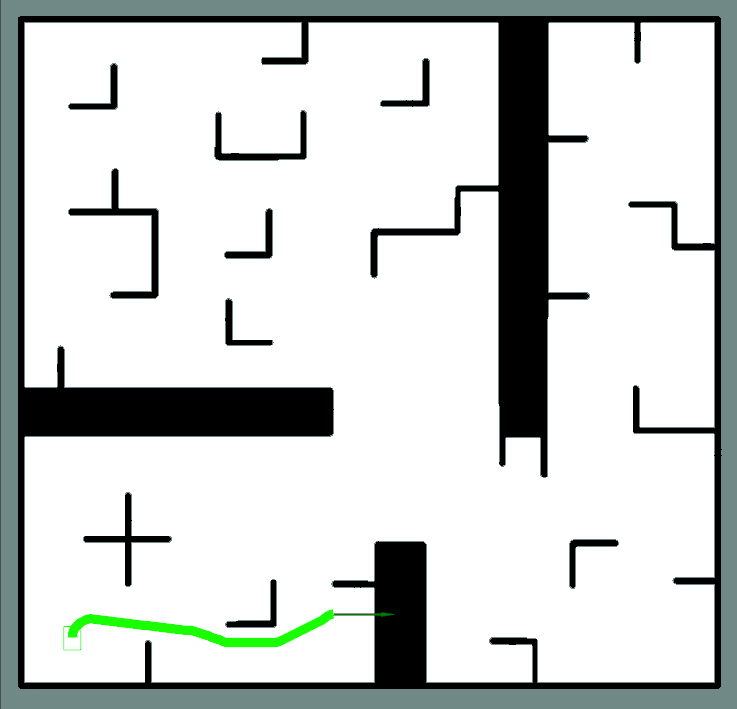
\includegraphics[width=0.24\linewidth]{Chapters/Chapter5/Figures/sbpl/arastar/so_arastar_p1.png}} \vspace{0.01\linewidth}
	\subfloat[$p_2$]{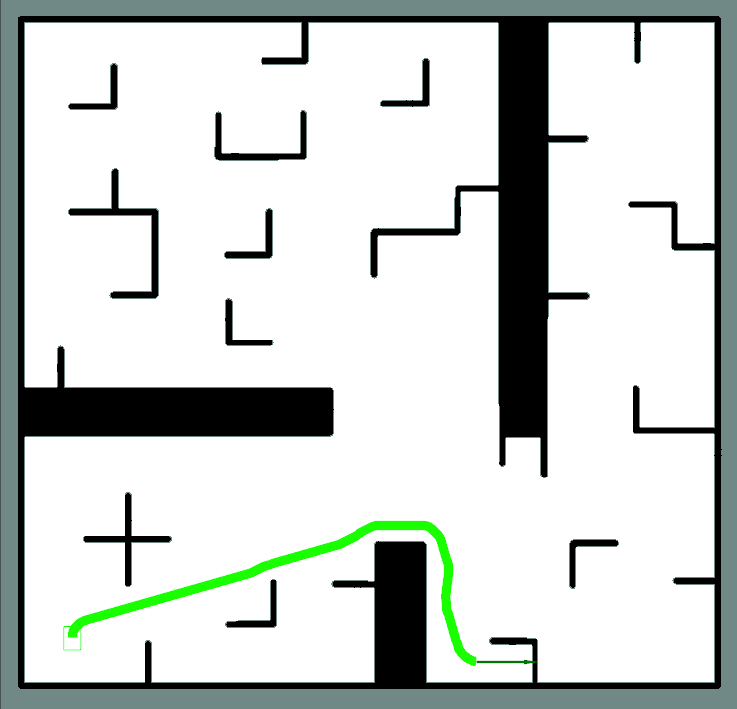
\includegraphics[width=0.24\linewidth]{Chapters/Chapter5/Figures/sbpl/arastar/so_arastar_p2.png}} \vspace{0.01\linewidth}
 	\subfloat[$p_3$]{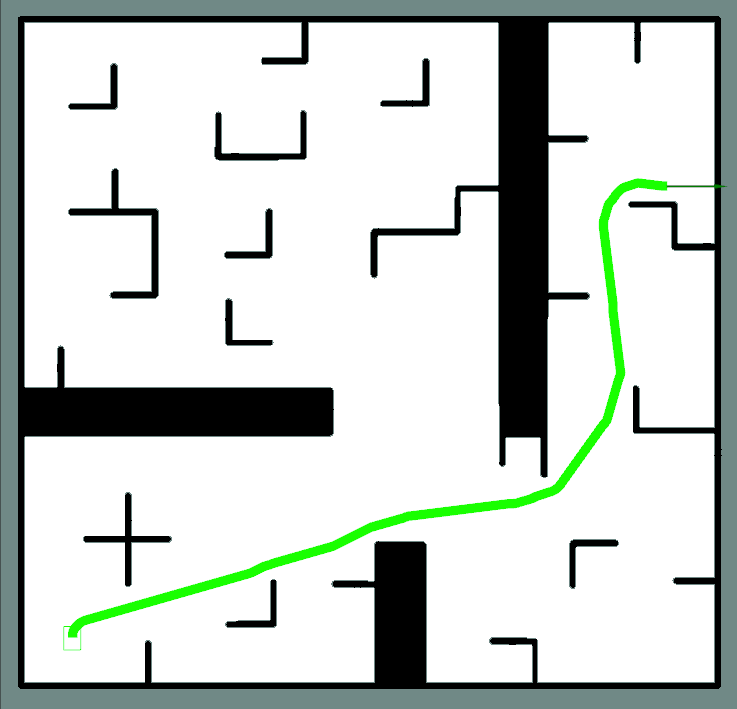
\includegraphics[width=0.24\linewidth]{Chapters/Chapter5/Figures/sbpl/arastar/so_arastar_p3.png}} \vspace{0.01\linewidth}
	\subfloat[$p_4$]{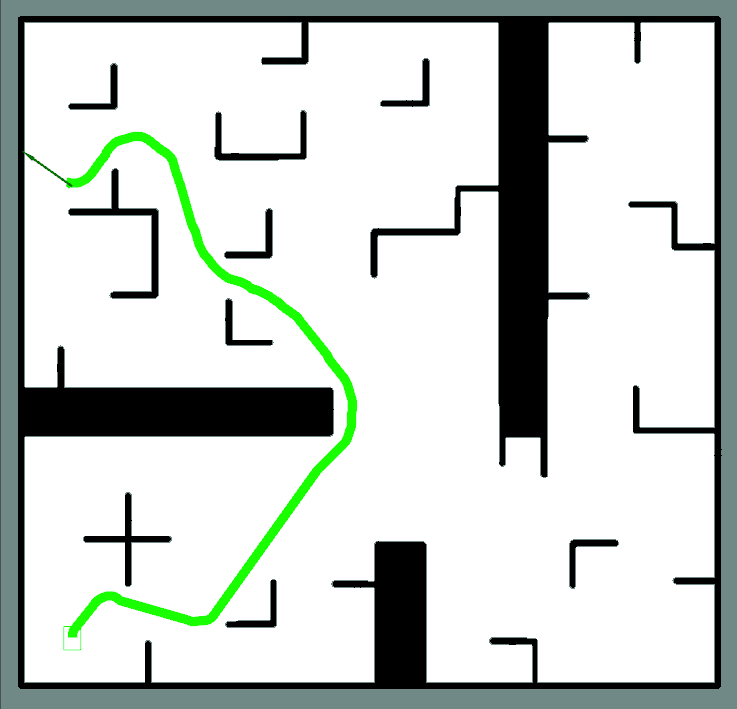
\includegraphics[width=0.24\linewidth]{Chapters/Chapter5/Figures/sbpl/arastar/so_arastar_p4.png}}\\[-0.25cm]
	\caption{Κατασκευή μονοπατιών με τον αλγόριθμο ARA*, για τις πόζες-στόχους $p_i$, $i=1,...,4$.} %Παρουσιάζονται τα τελικά βέλτιστα μονοπάτια και όχι τα αρχικά άκρως μη βέλτιστα.}
	\label{fig:arastar_experiments}
\end{figure}

\begin{figure}[!ht]
	\centering
	\subfloat[$p_1$]{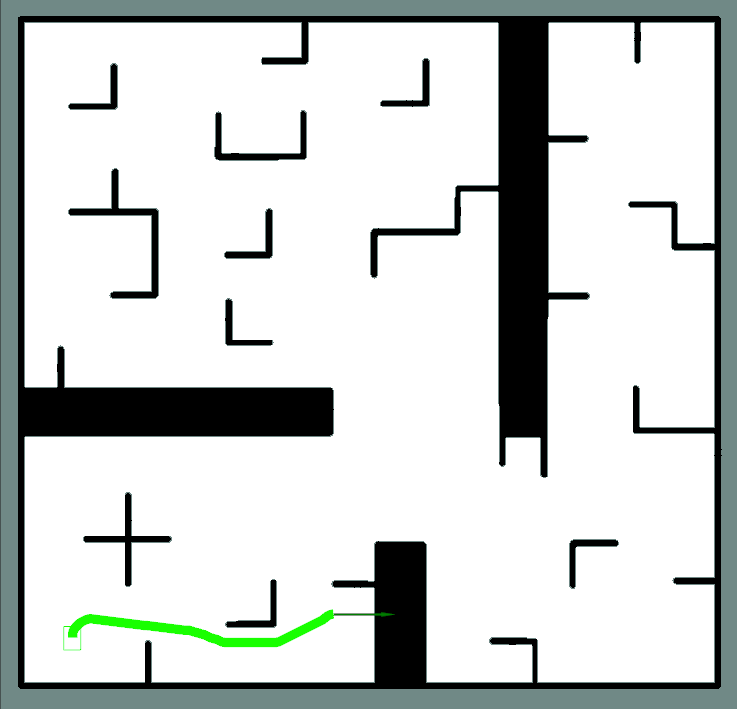
\includegraphics[width=0.24\linewidth]{Chapters/Chapter5/Figures/sbpl/adstar/so_adstar_p1.png}} \vspace{0.01\linewidth}
	\subfloat[$p_2$]{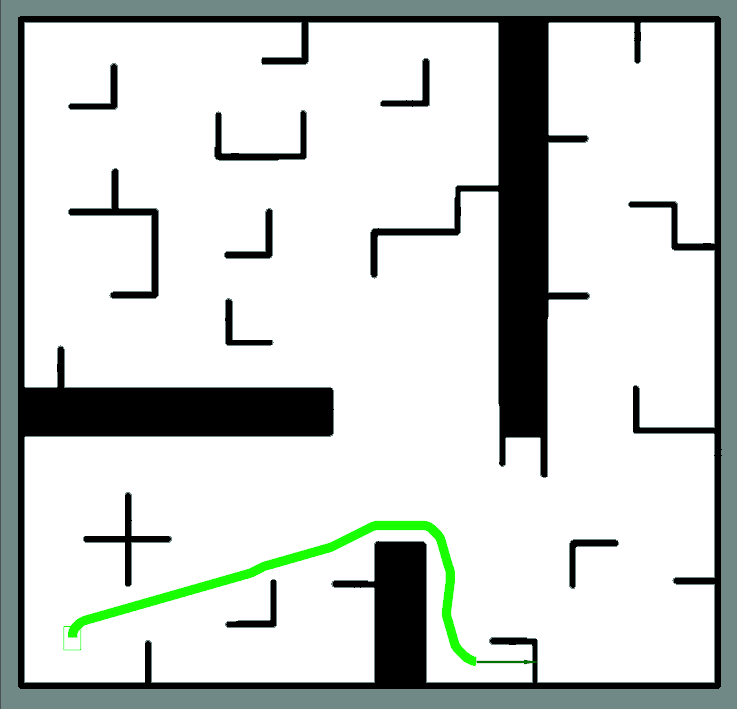
\includegraphics[width=0.24\linewidth]{Chapters/Chapter5/Figures/sbpl/adstar/so_adstar_p2.png}} \vspace{0.01\linewidth}
 	\subfloat[$p_3$]{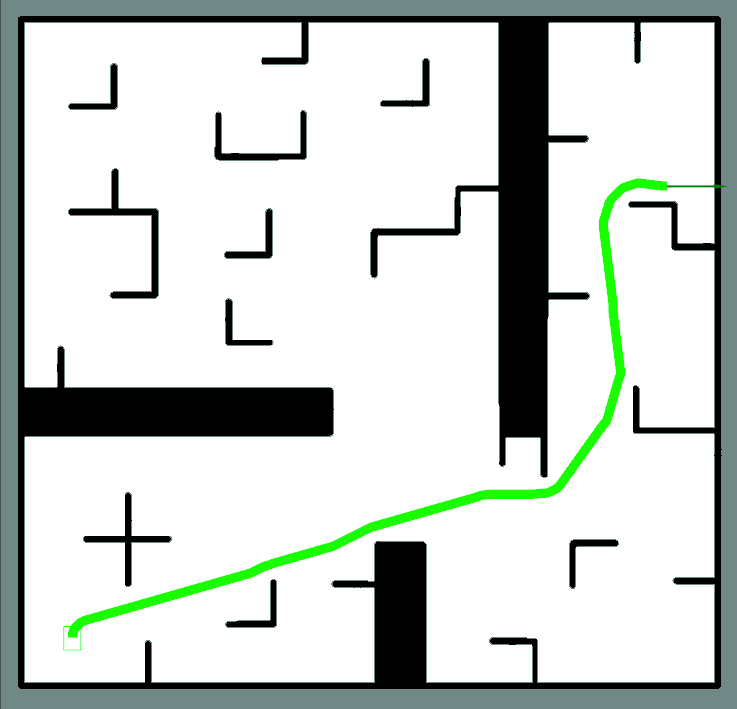
\includegraphics[width=0.24\linewidth]{Chapters/Chapter5/Figures/sbpl/adstar/so_adstar_p3.png}} \vspace{0.01\linewidth}
	\subfloat[$p_4$]{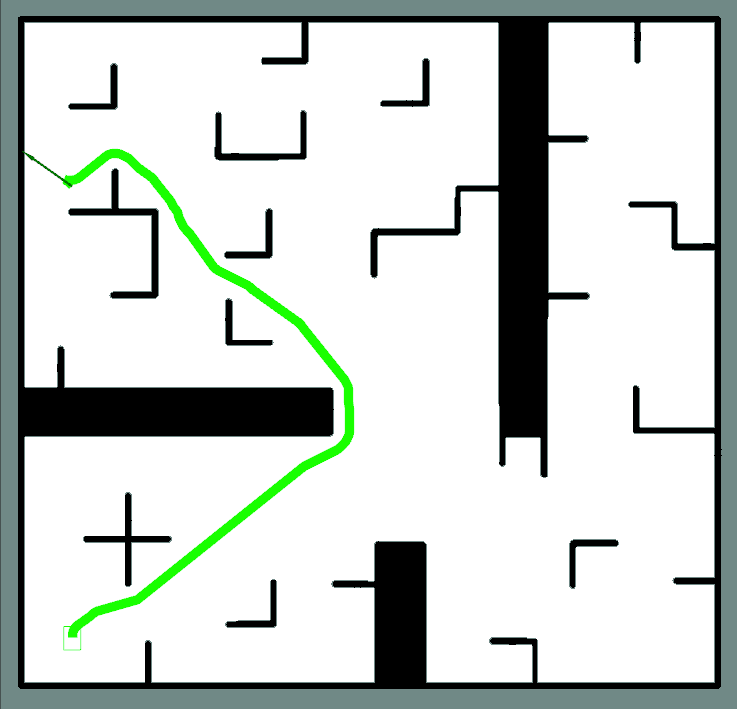
\includegraphics[width=0.24\linewidth]{Chapters/Chapter5/Figures/sbpl/adstar/so_adstar_p4.png}} \\[-0.25cm]
	\caption{Κατασκευή μονοπατιών με τον αλγόριθμο AD*, για τις πόζες-στόχους $p_i$, $i=1,...,4$.} %Παρουσιάζονται τα τελικά βέλτιστα μονοπάτια και όχι τα αρχικά άκρως μη βέλτιστα.}
	\label{fig:adstar_experiments}
\end{figure}

\begin{figure}[!ht]
	\centering
	\subfloat[$\epsilon_0=3$]{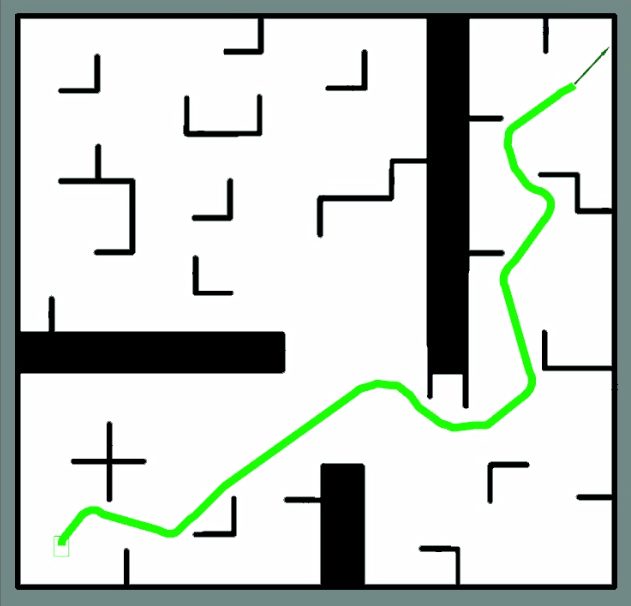
\includegraphics[width=0.24\linewidth]{Chapters/Chapter5/Figures/sbpl/arastar_successive_paths/so_arastar_v1.png}} \vspace{0.01\linewidth}
	\subfloat[$\epsilon_1: \epsilon_2<\epsilon_1<3$]{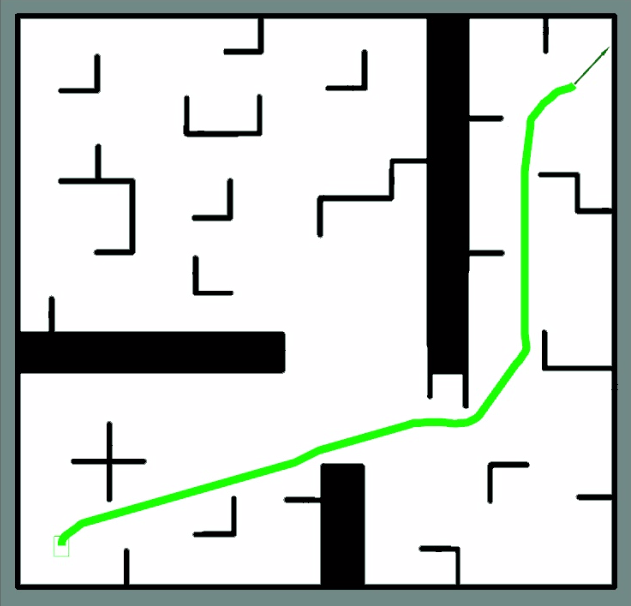
\includegraphics[width=0.24\linewidth]{Chapters/Chapter5/Figures/sbpl/arastar_successive_paths/so_arastar_v2.png}} \vspace{0.01\linewidth}
 	\subfloat[$\epsilon_2: 1<\epsilon_2<\epsilon_1$]{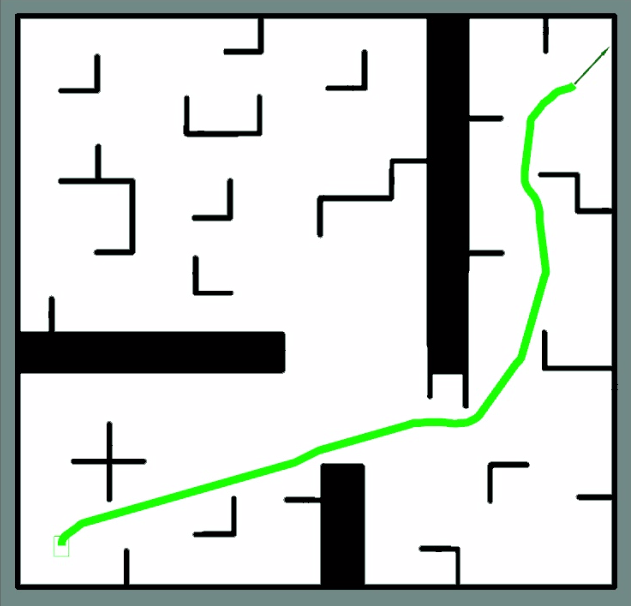
\includegraphics[width=0.24\linewidth]{Chapters/Chapter5/Figures/sbpl/arastar_successive_paths/so_arastar_v3.png}} \vspace{0.01\linewidth}
	\subfloat[$\epsilon_3=1$]{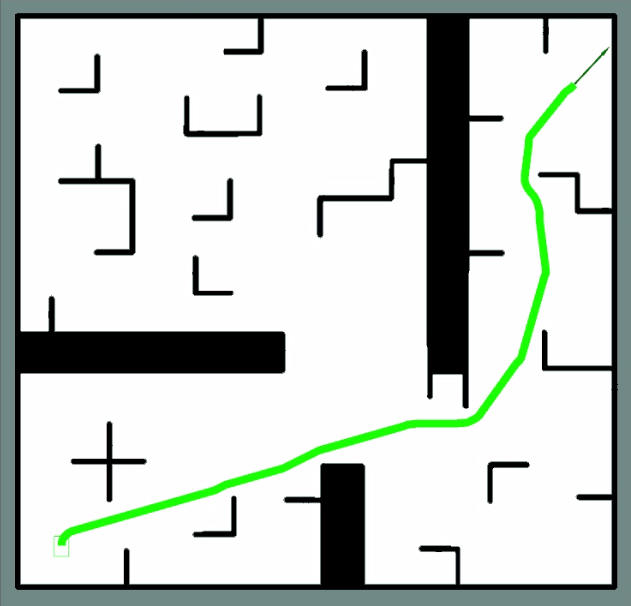
\includegraphics[width=0.24\linewidth]{Chapters/Chapter5/Figures/sbpl/arastar_successive_paths/so_arastar_v4.png}}\\[-0.25cm]
	\caption{Διαδοχική βελτιστοποίηση μονοπατιού με τον αλγόριθμο ARA*, για αυθαίρετο στόχο.}
	\label{fig:arastar_successive_paths_experiment}
\end{figure}

\begin{figure}[!ht]
	\centering
	\subfloat[$\epsilon_0=3$]{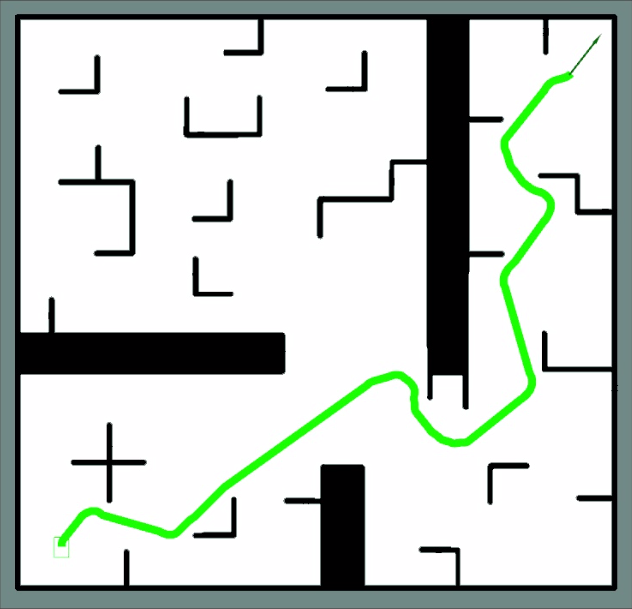
\includegraphics[width=0.24\linewidth]{Chapters/Chapter5/Figures/sbpl/adstar_successive_paths/so_adstar_v1.png}} \vspace{0.01\linewidth}
	\subfloat[$\epsilon_1: \epsilon_2<\epsilon_1<3$]{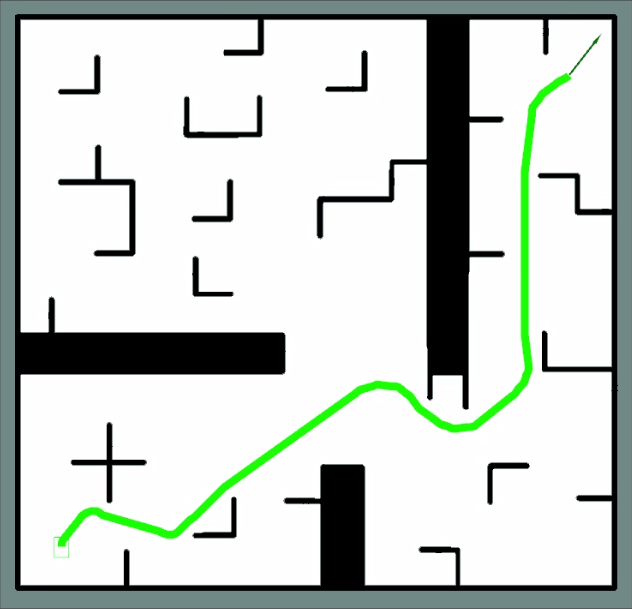
\includegraphics[width=0.24\linewidth]{Chapters/Chapter5/Figures/sbpl/adstar_successive_paths/so_adstar_v2.png}} \vspace{0.01\linewidth}
 	\subfloat[$\epsilon_2: 1<\epsilon_2<\epsilon_1$]{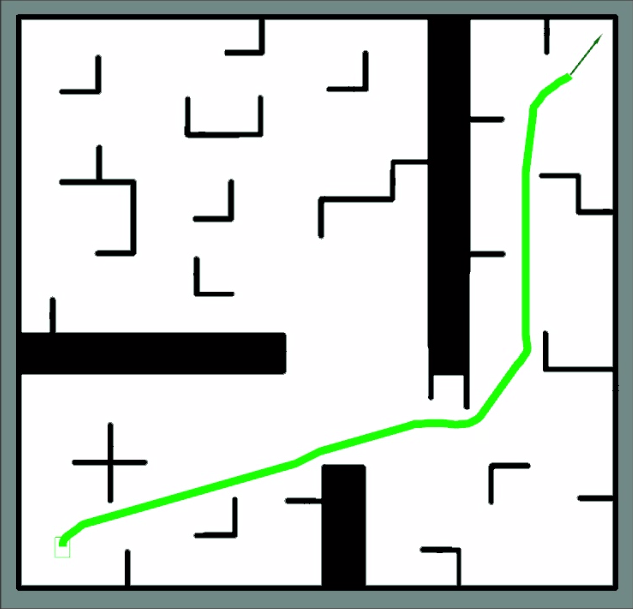
\includegraphics[width=0.24\linewidth]{Chapters/Chapter5/Figures/sbpl/adstar_successive_paths/so_adstar_v3.png}} \vspace{0.01\linewidth}
	\subfloat[$\epsilon_3=1$]{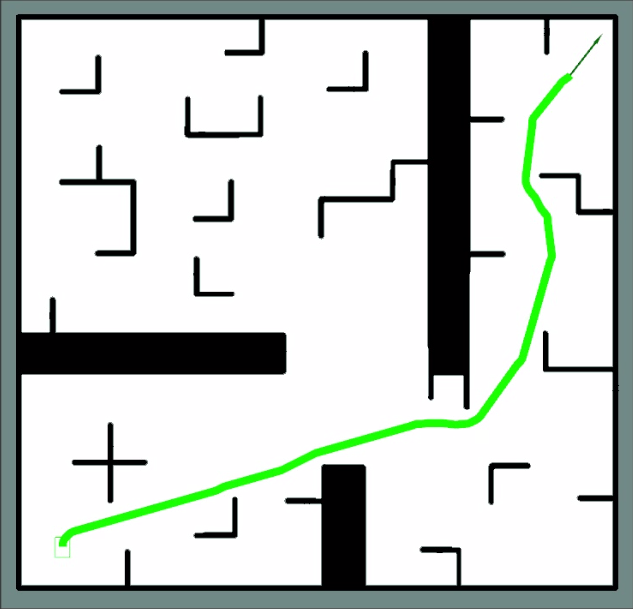
\includegraphics[width=0.24\linewidth]{Chapters/Chapter5/Figures/sbpl/adstar_successive_paths/so_adstar_v4.png}}\\[-0.25cm]
	\caption{Διαδοχική βελτιστοποίηση μονοπατιού με τον αλγόριθμο AD*, για αυθαίρετο στόχο.}
	\label{fig:adstar_successive_paths_experiment}
\end{figure}

\bigskip
\begin{table}[!ht]
\centering
\caption{Αποτελέσματα των πειραμάτων κατασκευής μονοπατιών.}
\label{tab:path_planning_experiments}
\begin{tabular}{|l|c|cc|cc|cc|cc|}
\cline{3-10}
\multicolumn{2}{l|}{}
& \multicolumn{2}{c|}{\textbf{Dijkstra}}                                                                  & \multicolumn{2}{c|}{\textbf{A*}}                                                                        & \multicolumn{2}{c|}{\textbf{ARA*}}                                                                               & \multicolumn{2}{c|}{\textbf{AD*}}                                                           \\ \cline{3-10} 
\multicolumn{2}{l|}{\multirow{-2}{*}{}}                                                                                & \multicolumn{1}{c}{\textbf{$T[s]$}} & \multicolumn{1}{c|}{\textbf{$s[m]$}} & \multicolumn{1}{c}{\textbf{$T[s]$}} & \multicolumn{1}{c|}{\textbf{$s[m]$}} & \multicolumn{1}{c}{\textbf{$s_{init}[m]$}} & \multicolumn{1}{c|}{\textbf{$s_{final}[m]$}} & \multicolumn{1}{c}{\textbf{$s_{init}[m]$}} & {\textbf{$s_{final}[m]$}} \\ \hline
\multicolumn{1}{|c|}{} & \textbf{$p_1$} & 0.035 & 6.02 & 0.027 & 6.02 & 6.68 & 5.91 & 7.45 & 5.92 \\ %\cline{2-2}
\multicolumn{1}{|c|}{} & \textbf{$p_2$} & 0.060 & 11.78 & 0.060 & 11.78 & 13.56 & 11.554 & 12.62 & 11.25  \\ 
\multicolumn{1}{|c|}{} & \textbf{$p_3$} & 0.110 & 19.34 & 0.090 & 19.34 & 19.85 & 18.73 & 23.26 & 18.66 \\
\multicolumn{1}{|c|}{\multirow{-4}{*}{\rotatebox[origin=c]{90}{\textbf{Στόχοι}}}} & \textbf{$p_4$} & 0.110 & 17.69 & 0.110 & 17.77 & 21.36 & 17.25 & 20.42 & 17.57 \\ \hline
\end{tabular}
\end{table}

\bigskip
Με βάσει τα παραπάνω αποτελέσματα κρίνεται ότι οι αλγόριθμοι Dijkstra και A* έχουν παραπλήσια συμπεριφορά, με τον αλγόριθμο Dijkstra να βρίσκει πάντα την βέλτιστη λύση, αλλά με τον αλγόριθμο A* να βρίσκει λύση σε μικρότερο χρόνο. Στην προκειμένη περίπτωση, εφόσον δεν υπάρχει σημαντικός περιορισμός στον χρόνο κατασκευής του μονοπατιού, μπορεί να χρησιμοποιηθεί οποιοσδήποτε από τους δύο αλγορίθμους, με προτίμηση στον αλγόριθμο Α*, λόγω του μικρότερου υπολογιστικού φόρτου, λόγω της πιο στοχευμένης αναζήτησης. Αντίστοιχα, όσον αφορά τους αλγορίθμους ARA* και AD* παρατηρείται, επίσης παραπλήσια στατική συμπεριφορά, και επομένως μπορεί να γίνει επιλογή μεταξύ οποιουδήποτε από τους δύο. Φυσικά, το πλεονέκτημα του AD*, έναντι του ARA* έγκειται στην δυναμική προσαρμογή του μονοπατιού σε περίπτωση που έχει αλλάξει  επαρκώς το περιβάλλον, λόγω ανίχνευσης νέων εμποδίων, δυναμικών ή μη.

\subsection{Παραμόρφωση Μονοπατιού με τον Αλγορίθμου Reeds-Shepp Band} \label{ssec:rsband_experiments}
Τα πειράματα παραμόρφωσης μονοπατιού με τον αλγόριθμο Reeds-Shepp Band πραγματοποιήθηκαν εξ ολοκλήρου στον 2D προσομοιωτή STDR, σε αραιό και πυκνό περιβάλλον, όσον αφορά τα εμπόδια. Συγκεκριμένα, χρησιμοποιήθηκαν τα περιβάλλοντα  \textit{simple{\_}rooms} και \textit{sparse{\_}obstacles} που παρέχονται από τον προσομοιωτή STDR και τα οποία παρουσιάζονται στο σχήμα \ref{fig:rsband_stdr_environments}. Επίσης, επιλέχθηκε να χρησιμοποιηθεί και πάλι ο έτοιμος χάρτης με ιδανικό εντοπισμό θέσης, χωρίς να εμπλέκεται το πρόβλημα της χαρτογράφησης και του εντοπισμού θέσης στην προκειμένη περίπτωση, ενώ, παράλληλα χρησιμοποιήθηκε σαρωτής λέιζερ με οπτικό πεδίο $360^o$, αντί για $240^o$ για την απαλοιφή άγνωστων τμημάτων στην νεκρό εύρος γωνιών του ρομπότ, του τοπικού χάρτη κόστους.

\begin{figure}[!ht]
	\centering
	\subfloat[simple{\_}rooms]{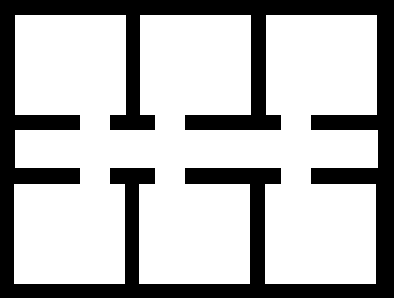
\includegraphics[height=5cm]{Chapters/Chapter5/Figures/simple_rooms.png}}
	\hspace{0.1\linewidth}
	\subfloat[sparse{\_}obstacles]{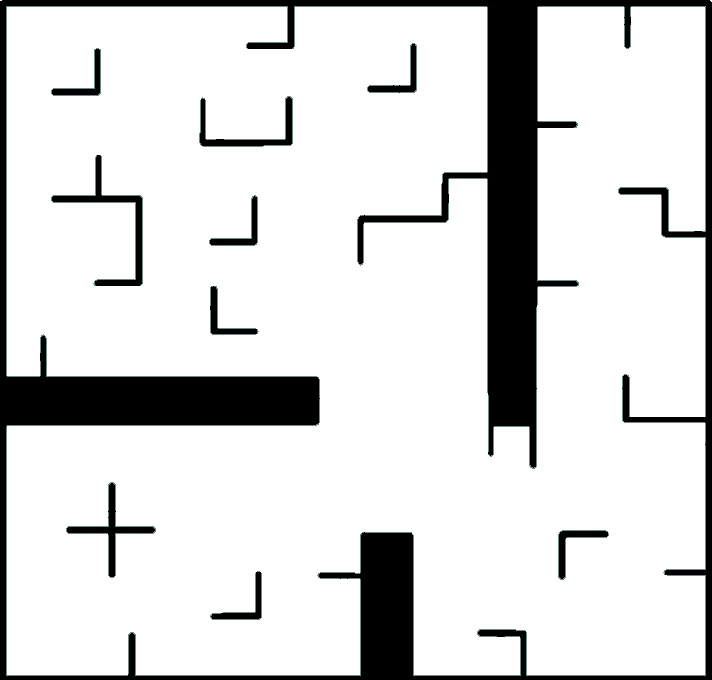
\includegraphics[height=5cm]{Chapters/Chapter5/Figures/sparse_obstacles.png}}
	\caption{Τα περιβάλλοντα του προσομοιωτή STDR που χρησιμοποιήθηκαν για τα πειράματα του αλγορίθμου Reeds-Shepp Band.}
	\label{fig:rsband_stdr_environments}
\end{figure}

\bigskip
Στόχος των πειραμάτων, της ενότητας αυτής, είναι η παρατήρηση της στατικής συμπεριφοράς του αλγορίθμου. Δηλαδή, το ρομπότ τοποθετείται σε προκαθορισμένες πόζες, χωρίς να κινείται και του δίνονται στόχοι χειροκίνητα, για την παραμόρφωση του ολικού μονοπατιού σε ελαστική ζώνη και την κατασκευή του αντίστοιχου τοπικού μονοπατιού, βάσει μονοπατιών Reeds-Shepp, όπου το ολικό μονοπάτι παράγεται μέσω του αλγορίθμου A* που υλοποιεί το plugin global{\_}planner. Επίσης, επιλέχθηκε να γίνει μετατροπή ολόκληρης της ελαστικής ζώνης σε ζώνη Reeds-Shepp μέσω ένωσης των ενδιάμεσων σημείων αυτής με μονοπάτια Reeds-Shepp και όχι μόνο των δύο πρώτων, για την καλύτερη αποτύπωση της συμπεριφοράς του αλγορίθμου.

\bigskip
Τα πρώτα πειράματα πραγματοποιήθηκαν στον ελεύθερο χώρο ενός δωματίου του περιβάλλοντος simple{\_}rooms, με στόχο την παρατήρηση της συμπεριφοράς του αλγορίθμου στον ελεύθερο χώρο, χωρίς την παρεμβολή εμποδίων. Επιλέχθηκαν συνολικά τέσσερις τυχαίες διαφορετικές πόζες ως στόχοι που δόθηκαν στο ρομπότ για την εξέταση της συμπεριφοράς του αλγορίθμου υπό διαφορετικές αντιπροσωπευτικές πιθανές περιπτώσεις. Τα αποτελέσματα των πειραμάτων αυτών, παρουσιάζονται στο σχήμα \ref{fig:simple_rooms_rsband}.

\begin{figure}[!ht]
	\centering
	\subfloat[Ολικό Μονοπάτι 1.]{\frame{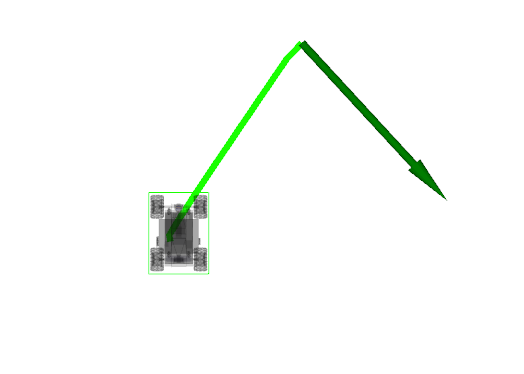
\includegraphics[width=0.275\linewidth]{Chapters/Chapter5/Figures/rsband/simple_rooms/rsband_global_1.png}}} \hspace{0.02\linewidth}
	\subfloat[Ελαστική Ζώνη 1.]{\frame{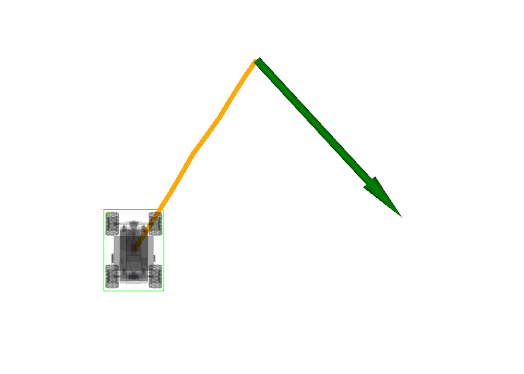
\includegraphics[width=0.275\linewidth]{Chapters/Chapter5/Figures/rsband/simple_rooms/rsband_eband_1.png}}}  \hspace{0.02\linewidth}
	\subfloat[Ζώνη Reeds-Shepp 1.]{\frame{\includegraphics[width=0.275\linewidth]{Chapters/Chapter5/Figures/rsband/simple_rooms/rsband_rsband_1.png}}}\\

	\subfloat[Ολικό Μονοπάτι 2.]{\frame{\includegraphics[width=0.275\linewidth]{Chapters/Chapter5/Figures/rsband/simple_rooms/rsband_global_2.png}}} \hspace{0.02\linewidth}
	\subfloat[Ελαστική Ζώνη 2.]{\frame{\includegraphics[width=0.275\linewidth]{Chapters/Chapter5/Figures/rsband/simple_rooms/rsband_eband_2.png}}} \hspace{0.02\linewidth}
	\subfloat[Ζώνη Reeds-Shepp 2.]{\frame{\includegraphics[width=0.275\linewidth]{Chapters/Chapter5/Figures/rsband/simple_rooms/rsband_rsband_2.png}}}\\

	\subfloat[Ολικό Μονοπάτι 3.]{\frame{\includegraphics[width=0.275\linewidth]{Chapters/Chapter5/Figures/rsband/simple_rooms/rsband_global_3.png}}} \hspace{0.02\linewidth}
	\subfloat[Ελαστική Ζώνη 3.]{\frame{\includegraphics[width=0.275\linewidth]{Chapters/Chapter5/Figures/rsband/simple_rooms/rsband_eband_3.png}}}  \hspace{0.02\linewidth}
	\subfloat[Ζώνη Reeds-Shepp 3.]{\frame{\includegraphics[width=0.275\linewidth]{Chapters/Chapter5/Figures/rsband/simple_rooms/rsband_rsband_3.png}}}\\

	\subfloat[Ολικό Μονοπάτι 4.]{\frame{\includegraphics[width=0.275\linewidth]{Chapters/Chapter5/Figures/rsband/simple_rooms/rsband_global_4.png}}} \hspace{0.02\linewidth}
	\subfloat[Ελαστική Ζώνη 4.]{\frame{\includegraphics[width=0.275\linewidth]{Chapters/Chapter5/Figures/rsband/simple_rooms/rsband_eband_4.png}}}  \hspace{0.02\linewidth}
	\subfloat[Ζώνη Reeds-Shepp 4.]{\frame{\includegraphics[width=0.275\linewidth]{Chapters/Chapter5/Figures/rsband/simple_rooms/rsband_rsband_4.png}}}\\

	\caption{Πειράματα παραμόρφωσης μονοπατιού με τον αλγόριθμο Reeds-Shepp Band σε ελεύθερο χώρο στο περιβάλλον simple{\_}rooms, όπου παρουσιάζονται το ολικό μονοπάτι (πράσινο), η ελαστική ζώνη (κίτρινο) και η ζώνη Reeds-Shepp (μωβ), για τέσσερις αυθαίρετες πόζες.}
	\label{fig:simple_rooms_rsband}
\end{figure}

\bigskip
Η δεύτερη κατηγορία πειραμάτων πραγματοποιήθηκε όμοια με την πρώτη, αλλά σε περιβάλλον πυκνό από εμπόδια, για την εξέταση της συμπεριφοράς του αλγορίθμου Reeds-Shepp Band, υπό την παρουσία εμποδίων. Τα αποτελέσματα παρουσιάζονται στο σχήμα \ref{fig:sparse_obstacles_rsband}.

\begin{figure}[!ht]
	\centering
	\subfloat[Ολικό Μονοπάτι 1.]{\frame{\includegraphics[width=0.275\linewidth]{Chapters/Chapter5/Figures/rsband/sparse_obstacles/rsband_global_1.png}}} \hspace{0.02\linewidth}
	\subfloat[Ελαστική Ζώνη 1.]{\frame{\includegraphics[width=0.275\linewidth]{Chapters/Chapter5/Figures/rsband/sparse_obstacles/rsband_eband_1.png}}}  \hspace{0.02\linewidth}
	\subfloat[Ζώνη Reeds-Shepp 1.]{\frame{\includegraphics[width=0.275\linewidth]{Chapters/Chapter5/Figures/rsband/sparse_obstacles/rsband_rsband_1.png}}}\\

	\subfloat[Ολικό Μονοπάτι 2.]{\frame{\includegraphics[width=0.275\linewidth]{Chapters/Chapter5/Figures/rsband/sparse_obstacles/rsband_global_2.png}}} \hspace{0.02\linewidth}
	\subfloat[Ελαστική Ζώνη 2.]{\frame{\includegraphics[width=0.275\linewidth]{Chapters/Chapter5/Figures/rsband/sparse_obstacles/rsband_eband_2.png}}} \hspace{0.02\linewidth}
	\subfloat[Ζώνη Reeds-Shepp 2.]{\frame{\includegraphics[width=0.275\linewidth]{Chapters/Chapter5/Figures/rsband/sparse_obstacles/rsband_rsband_2.png}}}\\

	\subfloat[Ολικό Μονοπάτι 3.]{\frame{\includegraphics[width=0.275\linewidth]{Chapters/Chapter5/Figures/rsband/sparse_obstacles/rsband_global_3.png}}} \hspace{0.02\linewidth}
	\subfloat[Ελαστική Ζώνη 3.]{\frame{\includegraphics[width=0.275\linewidth]{Chapters/Chapter5/Figures/rsband/sparse_obstacles/rsband_eband_3.png}}}  \hspace{0.02\linewidth}
	\subfloat[Ζώνη Reeds-Shepp 3.]{\frame{\includegraphics[width=0.275\linewidth]{Chapters/Chapter5/Figures/rsband/sparse_obstacles/rsband_rsband_3.png}}}\\

	\subfloat[Ολικό Μονοπάτι 4.]{\frame{\includegraphics[width=0.275\linewidth]{Chapters/Chapter5/Figures/rsband/sparse_obstacles/rsband_global_4.png}}} \hspace{0.02\linewidth}
	\subfloat[Ελαστική Ζώνη 4.]{\frame{\includegraphics[width=0.275\linewidth]{Chapters/Chapter5/Figures/rsband/sparse_obstacles/rsband_eband_4.png}}}  \hspace{0.02\linewidth}
	\subfloat[Ζώνη Reeds-Shepp 4.]{\frame{\includegraphics[width=0.275\linewidth]{Chapters/Chapter5/Figures/rsband/sparse_obstacles/rsband_rsband_4.png}}}\\

	\caption{Πειράματα παραμόρφωσης μονοπατιού με τον αλγόριθμο Reeds-Shepp Band, υπό την επίδραση εμποδίων, στο περιβάλλον sparse{\_}obstacles, όπου παρουσιάζονται το ολικό μονοπάτι (πράσινο), η ελαστική ζώνη (κίτρινο) και η ζώνη Reeds-Shepp (μωβ), για τέσσερις αυθαίρετες πόζες.}
	\label{fig:sparse_obstacles_rsband}
\end{figure}


\subsection{Πειράματα Αυτόνομης Πλοήγησης με Δυναμική Παραμόρφωση και Δυναμική Ανακατασκευή Μονοπατιού} \label{navigation_systems_comparison}
Στην παρούσα ενότητα παρουσιάζεται μία σύγκριση των δύο εξεταζόμενων συστημάτων αυτόνομης πλοήγησης με δυναμική παραμόρφωση μονοπατιού και δυναμική ανακατασκευή μονοπατιού, μέσω ορισμού στόχων και σύγκριση της απόκρισης κάθε συστήματος. Συγκεκριμένα, για την διεξαγωγή την πειραμάτων χρησιμοποιήθηκε ο προσομοιωτής STDR και το περιβάλλον sparse{\_}obstacles που χρησιμοποιήθηκε και σε προηγούμενα πειράματα, ενώ ως στόχοι ορίστηκαν οι πόζες που παρουσιάστηκαν στον πίνακα \ref{tab:path_planning_target_poses} και χρησιμοποιήθηκαν στο πειράματα κατασκευής μονοπατιών της ενότητας \ref{ssec:path_planning_experiments}.

\bigskip
Το ρομπότ τοποθετήθηκε στην ίδια πόζα $p_0=[1.5, 1.5, 90^o]$, με τα πειράματα κατασκευής μονοπατιών και καταγράφηκε η τροχιά που διάνυσε για κάθε έναν από τους τέσσερις στόχους και για τα δύο εξεταζόμενα συστήματα αυτόνομης πλοήγησης. Για την αξιολόγηση των πειραμάτων ορίστηκαν οι μετρικές $T_G$ και $s_G$ που δηλώνουν τον χρόνο που απαιτείται για την μετάβαση προς έναν δεδομένο στόχο και το μήκος της τροχιάς που διανύθηκε, αντίστοιχα. Στο σχήμα \ref{fig:dpm_experiments} παρουσιάζεται οι τροχιές που διάνυσε το ρομπότ για την μετάβαση από την αρχική του θέση προς κάθε έναν από τους τέσσερις στόχους, μέσω του συστήματος αυτόνομης πλοήγησης με δυναμικής παραμόρφωση μονοπατιού, ενώ στο σχήμα \ref{fig:dr_experiments} παρουσιάζονται οι αντίστοιχες τροχιές, βάσει του συστήματος δυναμικής ανακατασκευής μονοπατιού. Τέλος, στον πίνακα \ref{tab:navigation_experiments} παρουσιάζονται τα αποτελέσματα των παραπάνω πειραμάτων για κάθε ένα από τα εν λόγω συστήματα αυτόνομης πλοήγησης.

\begin{figure}[!ht]
	\centering
	\subfloat[$p_1$]{\includegraphics[width=0.24\linewidth]{Chapters/Chapter5/Figures/dpm/so_dpm_p1.png}} \vspace{0.01\linewidth}
	\subfloat[$p_2$]{\includegraphics[width=0.24\linewidth]{Chapters/Chapter5/Figures/dpm/so_dpm_p2.png}} \vspace{0.01\linewidth}
 	\subfloat[$p_3$]{\includegraphics[width=0.24\linewidth]{Chapters/Chapter5/Figures/dpm/so_dpm_p3.png}} \vspace{0.01\linewidth}
	\subfloat[$p_4$]{\includegraphics[width=0.24\linewidth]{Chapters/Chapter5/Figures/dpm/so_dpm_p4.png}}
	\caption{Αυτόνομη πλοήγηση με  δυναμική παραμόρφωση μονοπατιού, για μετάβαση στις πόζες-στόχους $p_i$, $i=1,...,4$.}
	\label{fig:dpm_experiments}
\end{figure}


\begin{figure}[!ht]
	\centering
	\subfloat[$p_1$]{\includegraphics[width=0.24\linewidth]{Chapters/Chapter5/Figures/dr/so_dr_p1.png}} \vspace{0.01\linewidth}
	\subfloat[$p_2$]{\includegraphics[width=0.24\linewidth]{Chapters/Chapter5/Figures/dr/so_dr_p2.png}} \vspace{0.01\linewidth}
 	\subfloat[$p_3$]{\includegraphics[width=0.24\linewidth]{Chapters/Chapter5/Figures/dr/so_dr_p3.png}} \vspace{0.01\linewidth}
	\subfloat[$p_4$]{\includegraphics[width=0.24\linewidth]{Chapters/Chapter5/Figures/dr/so_dr_p4.png}}
	\caption{Αυτόνομη πλοήγηση με δυναμική ανακατασκευή μονοπατιού, για μετάβαση στις πόζες-στόχους $p_i$, $i=1,...,4$.}
	\label{fig:dr_experiments}
\end{figure}

\bigskip
\begin{table}[!ht]
\centering
\caption{Αποτελέσματα των πειραμάτων αυτόνομης πλοήγησης με δυναμική παραμόρφωση μονοπατιού (DPM) και δυναμική ανακατασκευή μονοπατιού (DPR).}
\label{tab:navigation_experiments}
\begin{tabular}{|c|c|cc|cc|}
\cline{3-6}
\multicolumn{2}{c|}{} & \multicolumn{2}{c|}{\textbf{DPM}} & \multicolumn{2}{c|}{\textbf{DPR}} \\ \cline{3-6}

\multicolumn{2}{c|}{\multirow{-2}{*}{}} & \multicolumn{1}{c}{\textbf{$T_G[s]$}} & \multicolumn{1}{c|}{\textbf{$s_G[m]$}} & \multicolumn{1}{c}{\textbf{$T_G[s]$}} & \multicolumn{1}{c|}{\textbf{$s_G[m]$}} \\ \hline

\multicolumn{1}{|c|}{} & \textbf{$p_1$} & 38.80 & 6.93 & 35.2 & 6.06\\
\multicolumn{1}{|c|}{} & \textbf{$p_2$} & 65.00 & 12.23 & 63.20 & 11.6 \\ 
\multicolumn{1}{|c|}{} & \textbf{$p_3$} & 113.20 & 20.76 & 97.08 & 18.87 \\
\multicolumn{1}{|c|}{\multirow{-4}{*}{\rotatebox[origin=c]{90}{\textbf{Στόχοι}}}} & \textbf{$p_4$} & 102.20 & 19.06 & 98.20 & 17.57 \\ \hline
\end{tabular}
\end{table}

\bigskip
Βάσει του πίνακα \ref{tab:navigation_experiments}, προκύπτει ότι το σύστημα αυτόνομης πλοήγησης με δυναμική ανακατασκευή έφτασε στον επιθυμητό στόχο σε μικρότερο χρόνο και διάνυσε μικρότερη απόσταση από το σύστημα αυτόνομης πλοήγησης με δυναμική παραμόρφωση μονοπατιού. Το γεγονός αυτό, εξηγείται, αν παρατηρήσει κανείς ότι το σύστημα με δυναμική παραμόρφωση μονοπατιού κινήθηκε σε πιο ομαλή, αλλά και ασφαλέστερη τροχιά, δηλαδή πιο μακρυά από τα εμπόδια απ' ότι το πρώτο. Παράλληλα, αξίζει να σημειωθεί ότι το όχημα κινήθηκε με αρκετά χαμηλή ταχύτητα ($0.2m/s$), γεγονός που επέτρεψε την αξιόπιστη λειτουργία του συστήματος αυτόνομης πλοήγησης με δυναμική ανακατασκευή μονοπατιού, μέσω ανακατασκευής σε επαρκή συχνότητα. Αντίθετα, το σύστημα αυτόνομης πλοήγησης με δυναμική παραμόρφωση μονοπατιού, έχει δοκιμαστεί και με υψηλότερες ταχύτητες ($0.4-0.5m/s$) με αντίστοιχα αξιόπιστη συμπεριφορά.



%----------------------------------------------------------------------------------------
%	SECTION 4: Path Tracking Experiments
%----------------------------------------------------------------------------------------
\section{Πειράματα Διάσχισης Μονοπατιού} \label{sec:path_tracking_experiments}
Στην παρούσα ενότητα παρουσιάζονται τα πειράματα που πραγματοποιήθηκαν για την αξιολόγηση του αλγορίθμου διάσχισης μονοπατιού σε τρεις περιπτώσεις, υπό διαφορετικές συνθήκες. Το πρώτο πείραμα και πιο απλό πραγματοποιήθηκε σε μία πίστα με ομαλό έδαφος και διαδοχικά εμπόδια για την εξέταση της συμπεριφορά του αλγορίθμου, χωρίς την επίδραση φαινομένων ολίσθησης. Το δεύτερο πείραμα πραγματοποιήθηκε σε αντίστοιχη πίστα, αλλά με την προσθήκη ενός συνόλου από ράμπες για την προσέγγιση ανώμαλου εδάφους, με στόχο την εξέταση της συμπεριφοράς του αλγορίθμου υπό την επίδραση φαινομένων ολίσθησης. Τέλος, το τρίτο και τελευταίο πείραμα πραγματοποιήθηκε σε μία πίστα η οποία αποτελείται από έναν μακρόστενο διάδρομο με ομοιόμορφα κεκλιμένο επίπεδο για την εξέταση της συμπεριφοράς του αλγορίθμου υπό την επίδραση κάθετης πλευρικής ολίσθησης.

\bigskip
Για την πραγματοποίηση των πειραμάτων, χρησιμοποιήθηκε ο 3D προσομοιωτής Gazebo για την προσομοίωση των παραπάνω περιβαλλόντων. Επίσης, χρησιμοποιήθηκε το σύστημα χαρτογράφησης και εντοπισμού θέσης με τον αλγόριθμο SLAM και το σύστημα αυτόνομης πλοήγησης με δυναμική ανακατασκευή μονοπατιού, αλλά με σταθερό ολικό μονοπάτι σε συνδυασμό με τον αλγόριθμο διάσχισης μονοπατιού με ασαφή λογική.

\bigskip
Για την αξιολόγηση των πειραμάτων θα χρησιμοποιηθούν ως μετρικές, η ελάχιστη απόσταση $d_{RP}$ του ρομπότ από το μονοπάτι, όπως επίσης και το σφάλμα προσανατολισμού $E_o$ μεταξύ της πόζας του ρομπότ και της πόζας του τρέχοντος υπό-στόχου, πάνω στο μονοπάτι. Παράλληλα, θα παρουσιαστούν και τα σφάλματα θέσης $E_p$, απόκλισης γωνίας $E_a$, πλευρικής απόκλισης $E_y$, όπως επίσης και οι γωνίες στρέψης των τροχών καθ' όλη τη διάρκεια των πειραμάτων.

\subsection{Διάσχιση Μονοπατιού σε Ομαλό Έδαφος}
Για το πείραμα διάσχισης μονοπατιού σε ομαλό έδαφος σχεδιάστηκε και χρησιμοποιήθηκε το περιβάλλον \textit{zic{\_}zac{\_}room{\_}no{\_}ramps} που παρουσιάζεται στο σχήμα \ref{fig:zic_zac_room_no_ramps}. Για την πραγματοποίηση του εν λόγω πειράματος, εφόσον ο χάρτης του περιβάλλοντος δεν είναι εκ των προτέρων γνωστός, πραγματοποιήθηκε μία αρχική εξερεύνηση για την δημιουργία του πλήρους χάρτη του περιβάλλοντος και έπειτα πραγματοποιήθηκε το πείραμα για την μετάβαση από την μία πλευρά του χάρτη στην άλλη, με στόχο την παρακολούθηση της συμπεριφοράς του αλγορίθμου διάσχισης μονοπατιού. Στο σχήμα \ref{fig:zic_zac_room_no_ramps_path_and_traj} παρουσιάζονται το ολικό μονοπάτι που ακολούθησε το ρομπότ, όπως επίσης και η τροχιά που πραγματοποίησε για την επίτευξη του δεδομένου στόχου, ενώ στο σχήμα \ref{fig:zic_zac_room_no_ramps_errors} παρουσιάζονται τα σχετικά σφάλματα που προέκυψαν κατά την διάρκεια του πειράματος. Τέλος, στο σχήμα \ref{fig:zic_zac_room_no_ramps_fsa_rsa} παρουσιάζονται και οι γωνίες στρέψης των μπροστινών και πίσω τροχών του οχήματος καθ' όλη τη διάρκεια του πειράματος.

\begin{figure}[!ht]
	\centering
	\includegraphics[height=5cm]{Chapters/Chapter5/Figures/ptc_experiments/zic_zac_room_no_ramps.jpg}
	\caption{Το περιβάλλον \textit{zic{\_}zac{\_}room{\_}no{\_}ramps}}
	\label{fig:zic_zac_room_no_ramps}
\end{figure}	
	
\begin{figure}[!ht]
	\centering
	\includegraphics[height=5cm]{Chapters/Chapter5/Figures/ptc_experiments/zic_zac_room_no_ramps_path_and_traj.png}
	\caption{Ο χάρτης του περιβάλλοντος \textit{zic{\_}zac{\_}room{\_}no{\_}ramps}, το μονοπάτι που κλήθηκε να ακολουθήσει το ρομπότ (πράσινο) και η τροχιά που διάνυσε (κόκκινο).}
	\label{fig:zic_zac_room_no_ramps_path_and_traj}
\end{figure}

\begin{figure}[!ht]
	\centering
	\includegraphics[width=0.9\linewidth]{Chapters/Chapter5/Figures/ptc_experiments/plots/zic_zac_room_no_ramps/fsa_rsa.png}
	\caption{Διάγραμμα των εντολών στρέψης των τροχών κατά την πραγματοποίηση του πειράματος διάσχισης μονοπατιού στο περιβάλλον \textit{zic{\_}zac{\_}room{\_}no{\_}ramps}.}
	\label{fig:zic_zac_room_no_ramps_fsa_rsa}
\end{figure}

\begin{figure}[!ht]
	\centering
	\subfloat[$d_{RP}$]{\includegraphics[width=0.49\linewidth]{Chapters/Chapter5/Figures/ptc_experiments/plots/zic_zac_room_no_ramps/d_rp.png}}
	\subfloat[$E_o$]{\includegraphics[width=0.49\linewidth]{Chapters/Chapter5/Figures/ptc_experiments/plots/zic_zac_room_no_ramps/eo.png}}\\[1cm]
	\subfloat[$E_a$]{\includegraphics[width=0.49\linewidth]{Chapters/Chapter5/Figures/ptc_experiments/plots/zic_zac_room_no_ramps/ea.png}}
	\subfloat[$E_p$]{\includegraphics[width=0.49\linewidth]{Chapters/Chapter5/Figures/ptc_experiments/plots/zic_zac_room_no_ramps/ep.png}}\\[1cm]
	\subfloat[$E_y$]{\includegraphics[width=0.49\linewidth]{Chapters/Chapter5/Figures/ptc_experiments/plots/zic_zac_room_no_ramps/ey.png}}
	\caption{Διαγράμματα σφαλμάτων πειράματος διάσχισης μονοπατιού στο ομαλό περιβάλλον \textit{zic{\_}zac{\_}room{\_}no{\_}ramps}.}
	\label{fig:zic_zac_room_no_ramps_errors}
\end{figure}

\FloatBarrier

\subsection{Διάσχιση Μονοπατιού σε Ανώμαλο Έδαφος}
Για το πείραμα διάσχισης μονοπατιού σε ανώμαλο έδαφος σχεδιάστηκε και χρησιμοποιήθηκε το περιβάλλον \textit{zic{\_}zac{\_}room}, όπως αυτό παρουσιάζεται στο σχήμα \ref{fig:zic_zac_room}, ενώ το πείραμα εκτελέστηκε όμοια με το προηγούμενο. Στο σχήμα \ref{fig:zic_zac_room_path_and_traj} παρουσιάζεται το ολικό μονοπάτι που κλήθηκε να ακολουθήσει το ρομπότ, όπως επίσης και η τροχιά που πραγματοποίησε για την επίτευξη του δεδομένου στόχου, ενώ στο σχήμα \ref{fig:zic_zac_room_errors} παρουσιάζονται τα αντίστοιχα σφάλματα που προέκυψαν κατά την διάρκεια του πειράματος. Τέλος, στο σχήμα \ref{fig:zic_zac_room_fsa_rsa} παρουσιάζονται και οι γωνίες στρέψης των μπροστινών και πίσω τροχών του οχήματος καθ' όλη τη διάρκεια του πειράματος.

\begin{figure}[!ht]
	\centering
	\includegraphics[height=4.5cm]{Chapters/Chapter5/Figures/ptc_experiments/zic_zac_room.jpg}
	\caption{Το περιβάλλον \textit{zic{\_}zac{\_}room.}}
	\label{fig:zic_zac_room}
\end{figure}	
	
\begin{figure}[!ht]
	\centering
	\includegraphics[height=4.5cm]{Chapters/Chapter5/Figures/ptc_experiments/zic_zac_room_path_and_traj.png}
	\caption{Ο χάρτης του περιβάλλοντος \textit{zic{\_}zac{\_}room}, το μονοπάτι που κλήθηκε να ακολουθήσει το ρομπότ (πράσινο) και η τροχιά που διάνυσε (κόκκινο).}
	\label{fig:zic_zac_room_path_and_traj}
\end{figure}

\begin{figure}[!ht]
	\centering
	\includegraphics[width=0.9\linewidth]{Chapters/Chapter5/Figures/ptc_experiments/plots/zic_zac_room/fsa_rsa.png}
	\caption{Διάγραμμα των εντολών στρέψης τροχών κατά την πραγματοποίηση του πειράματος διάσχισης μονοπατιού στο περιβάλλον \textit{zic{\_}zac{\_}room.}}
	\label{fig:zic_zac_room_fsa_rsa}
\end{figure}

\begin{figure}[!ht]
	\centering
	\subfloat[$d_{RP}$]{\includegraphics[width=0.49\linewidth]{Chapters/Chapter5/Figures/ptc_experiments/plots/zic_zac_room/d_rp.png}}
	\subfloat[$E_o$]{\includegraphics[width=0.49\linewidth]{Chapters/Chapter5/Figures/ptc_experiments/plots/zic_zac_room/eo.png}}\\[1.25cm]
	\subfloat[$E_a$]{\includegraphics[width=0.49\linewidth]{Chapters/Chapter5/Figures/ptc_experiments/plots/zic_zac_room/ea.png}}
	\subfloat[$E_p$]{\includegraphics[width=0.49\linewidth]{Chapters/Chapter5/Figures/ptc_experiments/plots/zic_zac_room/ep.png}}\\[1.25cm]
	\subfloat[$E_y$]{\includegraphics[width=0.49\linewidth]{Chapters/Chapter5/Figures/ptc_experiments/plots/zic_zac_room/ey.png}}
	\caption{Διαγράμματα σφαλμάτων πειράματος διάσχισης μονοπατιού στο ανώμαλο περιβάλλον \textit{zic{\_}zac{\_}room.}}
	\label{fig:zic_zac_room_errors}
\end{figure}

\FloatBarrier

\subsection{Διάσχιση Μονοπατιού σε Κεκλιμένο Επίπεδο}
Για το πείραμα διάσχισης μονοπατιού σε κεκλιμένο επίπεδο σχεδιάστηκε και χρησιμοποιήθηκε το περιβάλλον \textit{slope{\_}room}, το οποίο αποτελείται από ένα μακρόστενο δωμάτιο με έδαφος που αποτελείται από ένα μικρό επίπεδο τμήμα στην αρχική θέση του ρομπότ και έπειτα έναν μακρύ διάδρομο με κλίση περίπου $15^o$. Το εν λόγω πείραμα εμπεριέχει την κίνηση κάθετα στον κεκλιμένο διάδρομο υπό την επίδραση ολίσθησης. Λόγω του μεγάλου μήκους του διαδρόμου, αλλά και την ομοιομορφία του περιβάλλοντος που δεν επιτρέπουν την αξιόπιστη χαρτογράφηση αυτού, επιλέχθηκε να αυξηθεί η εμβέλεια του σαρωτή λέιζερ στα 20m, έτσι ώστε να μπορεί να εντοπίσει το τέρμα της πίστας και να μπορεί έτσι το ρομπότ να αναγνωρίζει την θέση του αξιόπιστα. Στην συνέχεια, στο σχήμα \ref{fig:slope_room_path_and_traj} παρουσιάζεται το ολικό μονοπάτι που κλήθηκε να ακολουθήσει το ρομπότ, όπως επίσης και η τροχιά που πραγματοποίησε για την επίτευξη του δεδομένου στόχου, ενώ στο σχήμα \ref{fig:slope_room_errors} παρουσιάζονται τα σχετικά σφάλματα που προέκυψαν κατά την διάρκεια του πειράματος. Τέλος, στο σχήμα \ref{fig:slope_room_fsa_rsa} παρουσιάζονται και οι γωνίες στρέψης των μπροστινών και πίσω τροχών του οχήματος καθ' όλη τη διάρκεια του πειράματος.

\begin{figure}[!ht]
	\centering
	\includegraphics[width=\linewidth]{Chapters/Chapter5/Figures/ptc_experiments/slope_room.jpg}
	\caption{Το περιβάλλον \textit{slope{\_}room.}}
	\label{fig:slope_room}
\end{figure}	
	
\begin{figure}[!ht]
	\centering
	\includegraphics[width=\linewidth]{Chapters/Chapter5/Figures/ptc_experiments/slope_room_path_and_traj.png}
	\caption{Ο χάρτης του περιβάλλοντος \textit{slope{\_}room}, το μονοπάτι που κλήθηκε να ακολουθήσει το ρομπότ (πράσινο) και η τροχιά που διάνυσε (κόκκινο).}
	\label{fig:slope_room_path_and_traj}
\end{figure}

\begin{figure}[!ht]
	\centering
	\includegraphics[width=0.9\linewidth]{Chapters/Chapter5/Figures/ptc_experiments/plots/slope_room/fsa_rsa.png}
	\caption{Διάγραμμα των εντολών στρέψης τροχών κατά την πραγματοποίηση του πειράματος διάσχισης μονοπατιού στο περιβάλλον \textit{slope{\_}room.}}
	\label{fig:slope_room_fsa_rsa}
\end{figure}

\begin{figure}[!ht]
	\centering
	\subfloat[$d_{RP}$]{\includegraphics[width=0.49\linewidth]{Chapters/Chapter5/Figures/ptc_experiments/plots/slope_room/d_rp.png}}
	\subfloat[$E_o$]{\includegraphics[width=0.49\linewidth]{Chapters/Chapter5/Figures/ptc_experiments/plots/slope_room/eo.png}}\\[1cm]
	\subfloat[$E_a$]{\includegraphics[width=0.49\linewidth]{Chapters/Chapter5/Figures/ptc_experiments/plots/slope_room/ea.png}}
	\subfloat[$E_p$]{\includegraphics[width=0.49\linewidth]{Chapters/Chapter5/Figures/ptc_experiments/plots/slope_room/ep.png}}\\[1cm]
	\subfloat[$E_y$]{\includegraphics[width=0.49\linewidth]{Chapters/Chapter5/Figures/ptc_experiments/plots/slope_room/ey.png}}
	\caption{Διαγράμματα σφαλμάτων πειράματος διάσχισης μονοπατιού στο περιβάλλον, με κεκλιμένο επίπεδο, \textit{slope{\_}room.}}
	\label{fig:slope_room_errors}
\end{figure}

\FloatBarrier
%%%%%%%%%%%%%%%%%%%%%%%%%%%%%%%%%%%%%%%%%%%%%%%%%%%%%%%%%%%%%%%%%%%%%%%%%%%%%%%%%%%%%%%%%%%%

%----------------------------------------------------------------------------------------
%	SECTION 5: Exploration Experiments
%----------------------------------------------------------------------------------------
\section{Πειράματα Αυτόνομης Εξερεύνησης Πραγματικού Περιβάλλοντος} \label{exploration_experiments}
Στην παρούσα ενότητα, πραγματοποιούνται πειράματα αυτόνομης εξερεύνησης, χωρίς εκ των προτέρων  γνωστό περιβάλλον, μέσω των συστημάτων αυτόνομης πλοήγησης με δυναμική παραμόρφωση μονοπατιού (DPM) και δυναμική ανακατασκευή μονοπατιού (DPR), ενώ, για την χαρτογράφηση και τον εντοπισμό θέσης, χρησιμοποιείται ο αλγόριθμος CRSM-SLAM. Τα πειράματα εξερεύνησης πραγματοποιήθηκαν στον χώρο του Εργαστηρίου Αρχιτεκτονικής Υπολγιστών του τμήματος Ηλεκτρολόγων Μηχανικών και Μηχανικών Υπολογιστών του Αριστοτελείου Πανεπιστημίου Θεσσαλονίκης το οποίο παρουσιάστηκε στο σχήμα \ref{fig:csal}.

\bigskip
Για την αξιολόγηση των αποτελεσμάτων χρησιμοποιούνται οι μετρικές $T_{E}$ και $S_{E}$ που δηλώνουν τον χρόνο πλήρους εξερεύνησης του περιβάλλοντος και το μήκος της τροχιάς που διανύθηκε αντίστοιχα. Τα σχετικά αποτελέσματα παρουσιάζονται στο σχήμα \ref{fig:exploration_experiments} και στον πίνακα \ref{tab:exploration_experiments}.

\begin{figure}[!ht]
	\centering
	\subfloat[]{\frame{\includegraphics[height=7cm]{Chapters/Chapter5/Figures/exploration_dpm.png}}}
	\hspace{0.1cm}
	\subfloat[]{\frame{\includegraphics[height=7cm]{Chapters/Chapter5/Figures/exploration_dpr.png}}}
	\caption{Τροχιές που διανύθηκαν για την πλήρη εξερεύνηση του εργαστηρίου Αρχιτεκτονικής Υπολογιστών, μέσω των συστημάτων αυτόνομης πλοήγησης με (α')δυναμική παραμόρφωση μονοπατιού και (β')δυναμική ανακατασκευή μονοπατιού.}
	\label{fig:exploration_experiments}
\end{figure}

\bigskip
\begin{table}[!ht]
\centering
\caption{Αποτελέσματα των πειραμάτων αυτόνομης εξερεύνησης.}
\label{tab:exploration_experiments}
	\begin{tabular}{|c|c|c|}	\hline
		\cellcolor{gray} & $\mathbf{T_E[s]}$ & $\mathbf{S_E[m]}$\\ \hline
		\textbf{DPM} & $486$ & $114.89$\\ \hline
		\textbf{DPR} & $698$ & $93.38$\\ \hline
	\end{tabular}
\end{table}

Βάσει του πίνακα \ref{tab:exploration_experiments} παρατηρείται ότι το ρομπότ εξερεύνησε ταχύτερα τον χώρο, μέσω του συστήματος DPM, αλλά διάνυσε μεγαλύτερη συνολική απόσταση, από ότι μέσω του συστήματος DPR. Αυτό εξηγείται από το γεγονός ότι το σύστημα DPR απαιτεί περισότερο χρόνο για την κατασκευή μονοπατιών, με αποτέλεσμα να καθυστερεί η επιλογή στόχων, μέσω του συστήματος εξερεύνησης (exploration{\_}controller του πακέτου pandora{\_}explorer), καθώς αυτό απαιτεί την κατασκευή μονοπατιού για κάθε υποψήφιο στόχο, μέχρι να καταλήξει στην επιλογή ενός.

%%%%%%%%%%%%%%%%%%%%%%%%%%%%%%%%%%%%%%%%%%%%%%%%%%%%%%%%%%%%%%%%%%%%%%%%%%%%%%%%%%%%%%%%%%%%